
\chapter{基于自跳跃常微分方程网络的连续时间周期跳变系统建模}
周期跳变系统在现实生活中随处可见,其运行过程具有周期循环性。
连续时间周期跳变系统指各阶段依周期转换,
% 且每个周期内,各阶段之间按特定顺序进行切换。
且系统在不同阶段会呈现不同动态特性的连续时间跳变系统。
例如,洗衣机启动后将按程序设定,周期性地在进水,洗涤,排水,甩干等各个阶段之间循环运行,直至最后关机。
冰箱和空调在工作期间会在运行(压缩机开启)和待机(压缩机关闭)两种状态之间不断切换。
% 在一些自然界中其他的物理过程,也存在类似的系统,例如建筑物内的空调制冷系统、交通流量和季节变化等。
% 生产生活中的一些其他过程也存在类似特性,例如交通流量和季节变化等。
% % 在使用自回归模型对具有周期多阶段特性的系统进行预测时,我们希望模型能够自动地在特定时刻进行状态转移。
% 在对城市交通流量或某产品销量进行预测时,其流量或销量通常伴随着特定的日期和季节进行改变,并且其周期长度相对稳定,模型能够较容易地识别各时刻下被预测对象所处的当前阶段。
% 而对于一些复杂工业系统,其各阶段的持续时间可能受到系统内部和外部多个变量的影响。
% 例如系统的外部输入、当前内部状态、环境条件等。
% 为了优化此类系统的运行参数与运转模式,
利用历史数据建模其阶段跳变过程与各阶段内的动态模型参数对于优化此类系统的运行参数与运转模式是极其重要的。
% 对于此类带有多阶段特性的复杂工业系统,想要采用单一模型学习具有不同阶段特性的动态并且实现精确的系统预测与仿真是极其困难的。

然而,在对复杂跳变系统进行建模时会面临两大技术难题。
首先,跳变系统通常有多个阶段,每个阶段内系统将呈现完全不同的非线性特性,且各个阶段的持续时间可能同时受到内部因素和外部因素的影响\cite{WANG2022111790}。现有的跳变系统参数估计方法\cite{balenzuela2022parameter}通常依赖于对系统结构以及持续时间分布的先验认知,这需要大量的领域专家知识作为支撑。
另外,对于带有多输出项的工业系统,其输出项中可能同时存在稳定和非稳定过程\cite{nason2006stationary}。
目前为止,现有的未经过特定设计的辨识模型难以解决此类带有混合时序特性的系统学习任务。

% 为了实现上述目标,模型需要解决两个问题。
% 首先,模型需要根据系统的外部输入以及系统状态,识别在当前时刻系统所处的阶段。
% 另外,模型需要能够准确地识别系统在各阶段内的独立动态特性。
针对上述技术难题,本章提出了自跳跃常微分方程网络(Autonomous jump ordinary differential equation net, AJ-ODE-Net)以学习同时带有稳定和非稳定输出的连续时间周期跳变系统。
该模型是一种新颖的连续时间深度学习模型,能够从非均匀采样的系统历史轨迹进行学习。
% 该框架主要用于建模具有周期性多阶段转换的多输入输出系统,利用数据驱动的方式从系统输出序列中学习系统不同阶段的动态特性。
训练完成后,对于给定的系统外部输入,模型能够给出开环的仿真预测结果。
为了学习系统在不同阶段的动态特性,模型包含多个层次常微分方程网络(Hierarchical ODE-Nets ,H-ODE-Nets)。
该网络是一种双层扩展的常微分方程网络,能够建模同时带有稳定输出和非稳定输出的动态系统。
为了实现开环预测时的阶段自转移,本章对原始训练数据进行了阶段类别标注,并在模型中引入阶段转换预测器学习每个阶段的持续时间。
阶段转换预测器由多个持续时间预测器构成,每个预测器能够预估当前所处阶段的持续时间。在开环预测和仿真中,阶段转换预测器能够作为H-ODE-Nets的调节器,在每个时间点指派合适的H-ODE-Net进行系统输出的预测,并自发地转移至下一阶段。

% 为了使模型能够从数据中自动地学习各阶段内的系统动态特性,针对待预测系统输出同时存在非稳定过程和稳定过程的问题,引入分层常微分方程网络。
% (hierarchical ODE-Nets, H-ODE-Nets)实现对系统多维输出的混合学习。

% 因此,在本章提出的AJ-ODE-Nets模型中,参考了有限状态机的基本思想,构建了可学习的阶段转换模块。
同时为了给定AJ-ODE-Net的状态初值,
本章基于编码器解码器(Encoder-Decoder)框架,构建了两个AJ-ODE-Net分别用于历史数据的编码以及在给定的系统输入序列下以开环的方式预测系统的未来输出。
本章提出了基于编码器解码器(Encoder-Decoder)框架的预测模型。该模型包含两个AJ-ODE-Net,编码AJ-ODE-Net用于编码历史数据以给定解码AJ-ODE-Net的初态,解码AJ-ODE-Net能够在给定的系统输入序列下以开环的方式预测系统的未来输出。

% 除此之外,本章引入样条插值算法,以连续化离散的输入序列并作为AJ-ODE-Net模型的输入。
最后,本章将所述模型及编解码预测框架应用于具有典型周期多阶段特性的膏体制备水泥添加过程的预测与仿真问题中。
% 在给定系统的多变量输入数据下,包括热负载以及环境温度,模型能够仿真系统的运行过程并准确地预测系统能耗,能耗预测误差小于5\%。
在给定系统的多变量输入数据下,包括浓密机底流浓度以及底流流量,模型能够仿真系统的运行过程并准确地预测膏体浓度及水泥消耗,其中水泥量消耗量的预测误差小于5\%。
进一步地,利用模型的仿真功能能够优化膏体制备过程的浓度设定参数,仿真实验表明利用优化之后的浓度设定值能够在保证膏体浓度满足要求的前提下,显著减少螺旋给料器的开机频率以及水泥消耗6-25\%。
% 本章所述模型能够有效地模拟制冷系统的运行,预测其功率消耗以及服务器进气口温度。

% Addressing the challenges and problems mentioned above, we propose AJ-ODE-Nets, a novel framework for modeling and identifying the non-linear dynamics at different stages in periodic operational systems. The framework is specifically capable of capturing physical dynamics thanks to the implementation of ODE-Net, a neural network based on ODE. The framework is expected to learn the multivariate inputs-ouputs system in a data-driven way, by feeding several sequences of sensory data as training data. Once trained, the model is able to realize real time predictions according to the multivariate inputs. Modeling multi-stage periodic systems requires two principal realizations, one for the stages prediction, one for dynamical characteristics identifications of different stages. 





% With this purpose, in the design of AJ-ODE-Nets, a selective structure is considered.
% In terms of learning dynamical characteristics at different stages,
% the framework contains several hierarchical ODE-Nets (H-ODE-Nets), and the number depends on the observed system stages. H-ODE-Nets can be seen as an extension of ODE-Net, which can deal with both stationary and non-stationary sequences. 
% In terms of learning the system transitions during operation, a stage transition predictor is included in the AJ-ODE-Net module, which can infer the transfer actions from a sequence of observation data, specifically, when and how to change to other tendency during system operation. In order to train the stage transition predictor, the observation data has been labeled previously in a conditional data range, based on prior knowledge of the system operational specifications. During predictive range, the stage transition predictor serves as the governor to appoint to the suitable H-ODE-Net, so as to let the system run across different working stages periodically. Adaptive smoothing algorithm is introduced to impute missing data as well, it can handle nonlinear and irregularly sampling data, which is practical in dealing with sensory data from IoT systems. The AJ-ODE-Nets framework has been further implemented in a running data center with contained structure, to simulate the cooling system operations. 

本章研究主要包含三方面贡献,概括如下:
\begin{itemize}
    % \item 首先,本章将原始的ODE-Net模型扩展到H-ODE-Net模型,能够学习同时带有稳定和非稳定时间序列输出的动态过程。
    \item 为了辨识连续时间跳变系统,本章提出了一种新颖的深度学习模型——自跳跃常微分方程网络模型。该模型能够实现
    (1)在集成化的网络中学习系统的多阶段动态,(2)在长序列开环预测中实现阶段自转移。
    % \item 其次,本章针对具有周期多阶段特性的动态系统,开创性地提出了AJ-ODE-Nets模型,该模型通过引入阶段转换预测器学习系统的周期性阶段转换以及采用多个H-ODE-Nets学习不同阶段内的系统动态特性。
    \item 为了学习同时包含稳定和非稳定项的多输出系统,本章结合每个输出项的统计特性,引入H-ODE-Net以改善长期预测中两种输出项的预测精度。
    % \item 本章所述模型成功应用于某一工业制冷系统的预测与仿真问题中,该模型能够在给定热负载功率下,准确地预测制冷系统的功率消耗以及冷气温度变化,利用该仿真模型能够优化制冷系统的工作温度设定值,进而优化制冷系统整体能耗约6-25\%。
    \item 本章提出的AJ-ODE-Net模型成功应用于膏体制备系统的预测与仿真问题中,该模型能够在给定浓密机出料浓度与流量下,准确地预测系统的水泥消耗以及膏体浓度变化,利用该仿真模型能够优化控制螺旋给料器启停的浓度设定值,在控制螺旋给料器开机频率的同时,显著减少水泥消耗6-25\%。
\end{itemize}
% Two main contributions are devoted to this study, summarized as follows::
% \begin{itemize}
%     \item First, we extent the original vanilla ODE-Net to the Hierarchical ODE-Net (H-ODE-Net), which is able to learn the stationary and non-stationary time series data simultaneously.
%     \item Second, we propose AJ-ODE-Nets framework, targeting at learning periodic multi-states systems in data-driven way. AJ-ODE-Nets disposes of several H-ODE-Nets to automatically learn dynamic characteristics at different states, along with a stage transition predictor to learn the transition actions during operation. 
% \end{itemize}

本章正文内容的结构组织如下:
\ref{sec:4_notations}节给出了周期性多阶段系统预测问题中的变量符号定义以及形式化描述。
% 本章\ref{sec:h-ode}节介绍了分层常微分方程网络的定义及结构,以及如何将其用于学习同时带有稳定和非稳定时间序列输出的动态过程。
\ref{sec:4_ajode}节介绍了AJ-ODE-Net模型的基本结构,并详细阐述了
如何采用分层常微分方程网络学习同时带有稳定和非稳定时间序列输出的动态过程,以及如何构建连续时间域下的跳变系统状态转移方程。
% 最后给出了基于AJ-ODE-Net模型的编码器解码器框架及其训练方法
\ref{sec:4_encoder_decoder}节介绍了基于双AJ-ODE-Net模型的编码器解码器框架,并详细介绍了AJ-ODE-Net的初态求解方法。
\ref{sec:4_loss_function}节给出了用于训练持续时间预测器和预测模型的损失函数。
% 关键模块结构和持续时间预测器的损失函数定义等内容。
% 本章\ref{sec:4_encoder_decoder}给出了基于AJ-ODE-Net模型的编码器解码器框架及其训练方法。
\ref{sec:4_evalutaion}节将介绍利用所述框架建模膏体制备系统的水泥添加过程。
% 模型能够根据系统的热负载输入对其功耗以及出气口气体温度变化进行模拟预测,
同时,介绍如何利用辨识模型优化制备系统的浓度设定值以降低设备的重启频率并降低水泥消耗。
最后,\ref{sec:4_conclusion}节对本章工作进行总结,并对AJ-ODE-Net模型的未来研究方向以及在其他领域的应用做出了展望。


% The paper is organized as follows: related work on time series prediction for industrial systems, and for multi-state systems are summarized in Sec.~\ref{sec:review}. Then, preliminary in Sec.~\ref{sec:preliminary} describes the basic theory used in this study. After that, in Sec.~\ref{sec:methodology_dfaode}, the proposed framework AJ-ODE-Net is detailed in terms of data processing, structure of key modules and training for loss functions. In practice, the proposed framework is applied to simulate several working variables of a cooling system in real data centers. Two use cases are included, one for real time estimation of the energy consumption based on system inputs and environmental condition, and the other takes advantage of the integrated prior knowledge, simulations are conducted to optimize the consumption by varying configurations. In the end, Sec.~\ref{sec:4_conclusion} concludes the entire work and discuss the potential future work.
\section{问题形式化描述}
\label{sec:4_notations}
% 在本章中,标量和向量在形式上分别用小写字母和粗体小写字母表示,例如$y, \boldsymbol y$。
假设输入输出数据由传感器观测得到,并带有时间戳$t_i\in \mathbb{R}$。
因此,从系统中采集的带有非均匀采样间隔的离散输入序列和输出序列可表示为:
$\boldsymbol X_{1:I},\boldsymbol Y_{1:I}= ((t_1,\boldsymbol x_1,\boldsymbol y_1),(t_2,\boldsymbol x_2, \boldsymbol y_2),\cdots,(t_I,\boldsymbol x_I,\boldsymbol y_I))$。
%with each $t_i\in \mathbb{R}$ the timestamp of the system input and output, and $t_{0}<\cdots<t_{n}$.
% we define $\boldsymbol y_i$ as the $i$-th vectorial variable in a discrete sequence. 
相应的,定义$\boldsymbol x(t_i)=\boldsymbol x_i$ 以及 $\boldsymbol y(t_i)=\boldsymbol y_i$。
其连续时间过程可表示为$\boldsymbol x:\left[t_{1}, t_{I}\right] \rightarrow \mathbb{R}^{M}$ 和 $\boldsymbol y:\left[t_{1}, t_{I}\right] \rightarrow \mathbb{R}^{N}$。
为了便于后文描述,本章将$\boldsymbol y:\left[t_{1}, t_{I}\right]$简化为$\boldsymbol Y_{t_1:t_I}$。


连续时间跳变系统(Continuous-time Jump System,CTJS)由多个连续时间子系统组成,其内部阶段转换受有限状态过程控制\cite{8709809}。
典型的连续时间跳变系统定义如下:
% As an important class of dynamical systems, CTJS arises in many applications, such as failure prediction\cite{9165930}, control applications\cite{pmlr-v120-jansch-porto20a}, and state estimation\cite{8709809}.
% 作为一种特殊的动态系统,CTJS系统广泛应用于各类应用中,如故障预测\cite{9165930}、系统控制\cite{pmlr-v120-jansch-porto20a},以及状态估计\cite{8709809}。
\begin{equation}
    \dot{\boldsymbol h}(t)=\mathcal{F}_{\sigma(t)}(\boldsymbol h(t), \boldsymbol x(t),
    \label{equ:ctjls}
\end{equation}
% where $\sigma(t)\in\{0,1\cdots N-1\}$ is a finite-state step process and $\boldsymbol{x}(t)$ is system inputs with the Lipschitz continuity.
% With different $\sigma(t)$, the non-linear system dynamics $\mathcal{F}_{\sigma(t)}$ are distinct.
% Compared to a general continuous-time markov jump system whose state $\sigma(t)$ is a markov process, this study assumes that the transition of $\sigma(t)$ is deterministic and circular.
% Specifically, in a continuous-time periodic jump non-linear system, the piece wise constant state $\sigma(t)$ jumps in a cycle order $\{0,1,\cdots,N-1,0 \cdots\}$.
% The sojourn time between jumps depends on the trigger thresholds according to prior knowledge about the system.
% To distinguish between the state in a system and the hidden state in a recurrent neural network, we name the system state $\sigma(t)$ as the \textbf{\textit{stage} in this paper.
其中$\sigma(t)\in\{0,1\cdots,N-1\}$为一有限状态集下的跳变状态,$\boldsymbol{x}(t)$为满足利普希茨连续的系统输入。
为了明确区分跳变系统中的状态变量$\sigma(t)$以及循环神经网络中的隐状态,本章将跳变系统状态$\sigma(t)$命名为阶段。
在一般的连续时间马尔科夫跳变系统中,系统阶段$\sigma(t)$的变化遵循马尔科夫过程。
而本章假设阶段变量$\sigma(t)$的转移过程是依周期的且循环过程是确定的,
分段恒定的$\sigma(t)$在循环$\{0,1,\cdots,N-1,0 \cdots\}$中不断变化。
阶段跳跃之间的停留时间取决于由系统本体属性决定的触发条件。
因此本文所关注的系统也称为连续时间周期跳变系统(Continuous-time periodic jump system)。
% 基于模型驱动的参数估计或系统辨识方法有时很难被应用于复杂的跳跃系统中,因为实际的动态行为很难被识别。为了从现有的输入输出数据中学习CTJS,以前的研究假设了系统的先验结构,并采用了EM算法(balenzuela2022parameter}、顺序蒙特卡洛(SMC)(6859280)和变异推理(opper2007variational)等方法来估计模型参数。

同本文第三章,本章要解决的问题仍为根据系统的历史数据信息和以及系统的未来序列输入,开环地预测系统的未来输出。
具体地,本章将给定数据的时间范围$[t_1:t_{I+L}]$分为两部分:条件范围$[t_1:t_{I}]$和预测范围$[t_{I}:t_{I+L}]$。
%Given $\{{\boldsymbol{X}}_{t_{1}:t_{I+L}}, {\boldsymbol {Y}}_{t_{1}:t_{I+O}}\}$, the system inputs and system outputs in time range $[t_1:t_{I+O}]$,
% , where ${\boldsymbol y}^i_{1:I+O}=[{\boldsymbol y}^i(t_1),\boldsymbol y^i(t_2),\dots,{\boldsymbol y}^i(t_{I+O})]$ and ${\boldsymbol y}^i(t_j)$ is the $j-th$ value in $i-th$ system outputs series collected at time $t_j$ . 
模型通过给定条件范围$[t_1, t_I]$下的系统输入和系统输出生成初始状态,然后利用训练得到的跳变模型\equref{equ:ctjls}对预测范围$[t_{I}, t_{I+L}]$下的系统输出进行预测,如式~\ref{equa:problematique}所示:

\begin{equation}
\label{equa:problematique}
    \hat{\boldsymbol Y}_{t_{I}:t_{I+L}} = f(\boldsymbol Y_{t_{1}:t_{I}}, \boldsymbol X_{t_{1}:t_{I+L}};\boldsymbol \zeta) 
\end{equation}
公式中$\hat{\boldsymbol Y}_{t_{I}:t_{I+L}}$表示预测范围内的模型输出。 
$\boldsymbol Y_{t_{1}:t_{I}}$表示在条件范围内系统的历史输出。
$\boldsymbol X_{t_{1}:t_{I+L}}$表示完整时间范围内的系统输入,包括历史输入和未来输入部分,其未来输入也被称为协变量\cite{Wu2020}。
% 该系统输入在时间序列预测领域经常被称为协变量\cite{Wu2020}。
$\boldsymbol \zeta$表示利用数据集训练的模型可学习参数。
本章的目标为通过优化$\boldsymbol \zeta$以最小化$||\hat{\boldsymbol Y}_{t_{I}:t_{I+L}}-\boldsymbol {Y}_{t_{I}:t_{I+L}}||^2$。
值得注意的是,上述过程仍为开环预测,模型预测过程中无法收到来自系统输出的反馈。
% Where $\hat{\boldsymbol Y}_{t_{I}:t_{I+L}}$ is the estimated outputs in predictive range. $\boldsymbol Y_{t_{1}:t_{I}}$ represents the historical system outputs in conditional range.
% $\boldsymbol X_{t_{1}:t_{I+L}}$ is the system inputs of whole range that involve both historical and predictive parts.
% $\boldsymbol \zeta$ is the learnable parameters of model trained jointly from all available datasets. \\

% The formulation in Eq.~\eqref{equa:problematique} is similar to the time-series forecasting problem, which focuses on extracting temporal information and predicting the future outputs given historical observed targets and covariates \cite{Lim2021}.
% \eqref{equa:problematique}所示的形式化描述类似于时间序列预测问题。
% Time series forecasting methods are employed for extracting temporal information and predicting the future outputs given historical observed targets and covariates \cite{Lim2021}.
% However, the research scope of this paper is more related to the field of system modeling/identification , which focuses on modeling the dynamics of the system.
% The historical system observations herein are mainly utilized to provide an accurate initial state.
% With an inferred initial state, the model can predict the system outputs in open loop, based on the given system inputs in a predictive range. 
% The length of the predictive range is determined according to the length of the simulation we want to make.
% Taking the studied cooling system simulation as an example, we can theoretically feed arbitrary long heat loads as inputs and the model will simulate the corresponding temperature variation in that predictive range.
% 以制冷系统为例,可以将任意长度的热负载序列数据作为模型输入,模型能够仿真预测区间下的温度变化。
% 因此,在训练阶段,预测范围长度与条件范围长度是一致的,为800s。
% 在实验一中,预测范围的长度为30分钟,本章考虑到由于误差累积导致的相位偏差,因此没有采用点对点式的评估指标,而是采用预测累积能耗的估计误差对模型可靠性进行评估。

% However, when there is no feedback from system outputs, the long-term open-loop simulations are unreliable for a stochastic or uncertain system.
% In Section \ref{sec:case-study1}, although the length of the predictive range is altered to 30 minutes, 
% we considered the accumulated estimated error of phases positions and give up the point-to-point evaluation and seek other evaluation indicators


% \section{自跳跃常微分方程网络及编码器-解码器预测架构}
\section{自跳跃常微分方程网络}
\label{sec:4_ajode}
\subsection{基于分层ODE-Net的稳定及非稳定输出混合建模}
大部分工业系统的输出是多维度的,不同维度输出的时序统计特性存在一定差异,某些输出项为均值、方差恒定的稳定过程,某些输出项为均值、方差不断变化的非稳定过程。
对于同时含有稳定和非稳定输出的混合过程进行建模学习具有一定难度,当前主流的基于深度学习的序列预测领域并未针对该类系统开展研究。
针对该问题,本章提出分层常微分方程网络(Hierarchical ODE-Net, H-ODE-Net)以建模同时包含稳定过程和非稳定过程的复杂系统。

具体地,H-ODE-Net将三个ODE-Net集成为双层结构(L-1和L-2)。
% Modeling hybrid processes with both stationarity and non-stationarity properties is another challenge for industrial systems, as existing methods normally target one situation. With this in mind, Hierarchical ODE-Net (H-ODE) is proposed to model a system containing non-stationary and stationary processes simultaneously. In 图.~\ref{fig:AJ_ODEs}, there are $N$ number of H-ODE-Net embedded in the AJ-ODE-Net module, and only one will active at specific time point $t$, based on state variable $\sigma(t)$. In detail, H-ODE hierarchically integrates a two-level structure (L-1 and L-2) with three ODE-Nets.
% to deal with the mixed situations mentioned above.
%The learned continuous-time predictive model is named Hierarchical ODE-Net which hierarchically integrates a two-level ODE-Net.
图~\ref{fig:H_ode}展示了H-ODE-Net中三个ODE-Net之间的连接方式。
\begin{figure}
    \centering
    \includegraphics[width=\linewidth]{figures/chapter4/Hode.pdf}
    \caption{H-ODE-Net结构图示}
    %\caption{An H-ODE-Nets consists of three ODE-Net. The high-level ODE-Net estimates the derivative of latent state according to external inputs. By integrating the ODE equation with high-level ODE-Net, the solved $\boldsymbol h(t)$, accompanied with external inputs $\boldsymbol x(t)$ and duration time of current stage $T(t)$, is fed into two low-level ODE-Nets to estimate the derivatives of system outputs. The predictions of system outputs at arbitrary time points $t_x$ can be solved by integrating the low-level ODE-Nets.}
    \label{fig:H_ode}
\end{figure}
在L-1层中的一个ODE-Net用于根据外部输入对隐状态的导数进行建模。利用实时求解出的$\boldsymbol h(t)$、外部输入$\boldsymbol x(t)$和当前阶段持续时间$T(t)$,对由L-1中的ODE-Net定义的常微分方程进行积分。
在L-1层中的一个ODE-Net
用于根据外部输入对隐状态的导数进行建模。
利用实时求解出的$\boldsymbol h(t)$、外部输入$\boldsymbol x(t)$和当前阶段持续时间$T(t)$对隐状态导数进行建模。
% 由L-1中的ODE-Net定义的常微分方程进行积分。
对L-1中定义的常微分方程进行积分解出的$\boldsymbol h(t)$将作为L-2中两个ODE-Net的输入,并分别用于求解稳定系统输出项和非稳定系统输出项,表示为$\boldsymbol y(t)=[\boldsymbol y_s(t), \boldsymbol y_{ns}(t)]$。
% 最终,可以解出任一时间点$t_x$下的预测结果。

% 图.~\ref{fig:H_ode} illustrates the connections between three ODE-Nets within H-ODE. The L-1 contains one ODE-Net to model the derivative of
% %The high level part of H-ODE-Net is an ODE-Net that 
% latent state according to external inputs. By integrating the ODE equation with ODE-Net of L-1, the solved $\boldsymbol h(t)$, combined with external inputs $\boldsymbol x(t)$ and duration of current stage $T(t)$, are fed into L-2 ODE-Nets to model the derivatives of stationary and
% %the stationary system outputs and 
% non-stationary system outputs, denoted as $\boldsymbol y(t)=[\boldsymbol y_s(t), \boldsymbol y_{ns}(t)]$ respectively. The predictions at arbitrary time points $t_x$ are solved in the end. 
%and the low-level part consists of 
%and only one particular H-ODE-Net corresponding to $s(t)$ may be utilized to make prediction at time point $t$.
%To utilize one model to predict a system involving the non-stationary and stationary process simultaneously, we propose a hierarchical ODE-Net whose three ODE-Nets predict the derivative of latent state, the derivative of stationary system outputs and the derivative of non-stationary system outputs respectively.

其中,L-1中的ODE-Net为第三章所述的稳定结构,由门控循环单元(GRU)网络实现:
% The ODE-Net in L-1
% %for modeling latent state 
% is stationary and implemented by stationary Gate Recurrent Unit (GRU) network\cite{Demeester2019}:
\begin{equation}
    \label{equ:dh}
    \frac{d \boldsymbol{h}(t)}{dt} = \frac{1}{\mu(t)}*\left[\text{GRU}(\boldsymbol{x}(t), \boldsymbol{h}(t),\text{sigmoid}(T(t)), \theta^\mathcal{H}_{\sigma(t)}) - \boldsymbol{h}(t)\right]
\end{equation}
其中$\mu(t)$表示原始数据集的平均采样间隔均值。
稳定的GRU网络将预测的隐状态变量$\boldsymbol{h}(t)$的变化表示为稳定过程,并将其上下界限制在$(-1,1)$范围内。


% where $\mu(t)$ denotes the mean of sampling intervals in entire dataset.
% Stationary GRU network treats the predicted latent state $\boldsymbol{h}(t)$ as a stationary process and constrains the outputs within range $(-1,1)$. 
% In comparison to stationary model which produces stabilized latent state, incremental models(non-stationary model) suffers from potentially linearly growing state, which is ill-suited for modeling long-term stationary time series~\cite{Demeester2019}.

% unit root problem and bring in long-term prediction.
% potentially linearly growing state is ill-suited for modeling stationary time series
%The low-level ODE-Nets

L-2中的两个ODE-Net被分别用于建模稳定和非稳定的系统输出。
其中被用于建模非稳定输出的导数网络采用非稳定增量形式预测输出$y_{ns}(t)$ :

% The two ODE-Nets in L-2 are designed to %is utilized to model the instant derivatives for system outputs in using two ODE-Nets 
% cover both stationary and non-stationary cases.
% % In this study, consumed power of cooling system $y_1(t)$ and cooling capacity $y_2(t)$ are categorized as stationary outputs, $\boldsymbol{y}_{s}(t)=[y_1(t), y_2(t)]^T$.
% % The inlet temperature of cooling system $y_3(t)$ is categorized as non-stationary outputs, $\boldsymbol{y}_{ns}(t)=[y_3(t)]^T$. 
% The one for $y_{ns}(t)$ is employed by implementing non-stationary incremental neural network:
% %One of low-level ODE-Nets, implemented by an non-stationary incremental neural network, is employed to model non-stationary outputs:
\begin{equation}
    \label{equ:dyns}
    \frac{d \boldsymbol{y}_{ns}(t)}{dt} = \text{NN}(\boldsymbol{x}(t),\boldsymbol{y}_{ns}(t), \boldsymbol{h}(t), \text{sigmoid}(T(t)), \theta^{\mathcal{Y}^{ns}}_{\sigma(t)})
\end{equation}

另一个ODE-Net类似于L-1中的ODE-Net,由稳定的GRU模型构建,用于预测系统的稳定输出$y_s(t)$:
% Another ODE-Net for $y_s$ is similar with the one in L-1, which is implemented by a stationary GRU module
% to model stationary outputs:
\begin{equation}
    \label{equ:dys}
    \frac{d \boldsymbol{y}_{s}(t)}{dt} = \frac{1}{\mu(t)}*\left[\text{GRU}(\boldsymbol{x}(t),\boldsymbol{y}_s(t), \boldsymbol{h}(t), \text{sigmoid}(T(t)), \theta^{\mathcal{Y}^{s}}_{\sigma(t)}) - \boldsymbol{y}_s(t)\right]
\end{equation}

对于L-2中的两个ODE-Net,均将系统处于当前阶段的持续时间$T(t)$作为特征输入,辅助估计 $\boldsymbol{y}(t)$的导数。
$\{\theta_i^{\mathcal{Y}^{ns}},\theta_i^{\mathcal{Y}^{ns}},\theta_i^{\mathcal{H}}\}_{i=1}^N$是模型中的可学习参数。
% In both L-1 and L-2, duration of current stage $T(t)$, accumulated since the start of each stage, is chosen as a feature to estimate the derivatives of $\boldsymbol{y}(t)$. 
% $\{\theta_i^{\mathcal{Y}^{ns}},\theta_i^{\mathcal{Y}^{ns}},\theta_i^{\mathcal{H}}\}_{i=1}^N$ are learnable parameters.
%because the periodic system has similar behaviors in the same stages and similar time points.
% employed to model stationary outputs and non-stationary outputs separately:
% hypothesize that it is there- fore more naturally suited to deal with stationary data.
% Two low-level ODE-Nets are 

一般情况下,从传感器测量得到的数据通常是离散的且带有不规则分布的缺失值。例如可能存在某一时刻$i$,两区间$t_i-t_{i-1} \neq t_{i+1}-t_{i}$或者存在$\boldsymbol x(t_i)$存在,而$\boldsymbol y(t_i)$缺失的情况。
本章采用第三章\ref{sec:3_interpolation_training}中介绍的并行可微插值方法,将离散的控制输入序列插值为连续时间信号并作为ODE-Net的输入。
% 因此需要实现面向离散序列输入的连续化插值方法,将离散和采样不规则的数据格式转换为连续时间格式。
% 为了实现该目标,有多种方法可以实现,如高斯过程\cite{li2016scalable},核方法\cite{shukla2018interpolation}或样条插值\cite{kidger2020neural}。本章参考\cite{kidger2020neural}采用三次样条插值方法。
% Generally speaking, data samples got from sensory measure system are commonly discrete and irregularly distributed with proportional missing values. 
% It may exist one timestamp $i$, the interval $t_i-t_{i-1} \neq t_{i+1}-t_{i}$, or $\boldsymbol x(t_i)$ exists while $\boldsymbol y(t_i)$ is missing and be represented as \textit{Null} in dataset.
% % As an instance, some
% ODE-Net takes only continuous data as input, therefore, the processing module is in charge of implementing interpolation methods to transfer discrete and irregular data samples to continuous format. There are many options, such as Gaussian processes\cite{li2016scalable}, kernel methods\cite{shukla2018interpolation} or natural cubic spline \cite{kidger2020neural}, appropriate interpolation method is free to apply in consideration of concrete situations.



% \subsection{基于循环神经网络的初始状态编码}
\subsection{微分方程状态空间定义及阶段自转移}
% \label{sec:dfa-odenet}
% \subsection{状态定义}
% 部分工业系统存在多阶段、非确定和多物理过程混合等复杂特性。对这类系统进行高精度、高鲁棒的建模是一项具有挑战性的任务。
% 在本章研究中,为了能够使模型准确地预测多阶段系统的阶段转换时刻以及预测系统输出,本章提出了AJ-ODE-Net模型。
为了使辨识模型准确地预测周期跳变系统中的阶段转换以及建模各个阶段下的系统输出,本节在H-ODE-Net基础上提出了自跳跃常微分方程网络模型。
具体地,我们首先利用系统先验知识构建系统的多阶段转换过程,对于每个阶段引入一个H-ODE-Net以学习系统在该阶段内的动态特性,通过对训练集中的序列数据进行阶段变量标注,可以定向地训练各个H-ODE-Net的参数。
同时,在预测框架中引入阶段转换预测器学习预测每个阶段的持续时间。
在测试阶段,阶段预测器可以作为不同H-ODE-Net的调节器,实现不同阶段之间的自动转移。
图~\ref{fig:AJ_ODEs}简要介绍了AJ-ODE-Net的主要组件及其结构。
\begin{figure}
    \centering
    \includegraphics[width=0.9\textwidth]{figures/chapter4/Jump-ODEnet.pdf}
    \caption{AJ-ODE-Net 模型结构}
    \label{fig:AJ_ODEs}
\end{figure}

在图\ref{fig:AJ_ODEs}中,AJ-ODE-Net模型嵌入了$N$个H-ODE-Net模块,根据状态变量$\sigma(t)\in \{0,\cdots,N-1\}$,在同一时刻只使用一个H-ODE-Net用于系统预测。
相比于普通的ODE-Net仅建模系统隐状态的导数,
AJ-ODE-Net将隐状态扩展为四个参数,即$\boldsymbol{S}(t) = [\boldsymbol h(t), \boldsymbol y(t), \sigma(t), T(t)]$,
其中四项分别为\textbf{系统隐状态}、\textbf{预测的系统输出}、\textbf{系统所处的当前阶段}和\textbf{处于当前阶段已经持续的时间}。
这种定义形式能够覆盖连续时间跳变系统中建模系统输出变化以及阶段变量变化所需的全部信息。
AJ-ODE-Net可以看作是ODE-Net的扩展形式,其状态的计算与更新均在连续时间域下进行。
给定时间点$t$和无穷小时间步长$\tau$,状态更新方程
如\equref{equ:stage_trans_predic}所示:

% For attention, even though there are several ODE-Nets as dynamical representations for available stages, only one ODE-Net is active during processing, appointed by stage predictor. Therefore, AJ-ODE-Net can still be seen as an extended version of ODE-Net. Different to ODE-Net shown in 式 \eqref{equ:ode_net} , which contains only self-governed hidden state predicted from input, AJ-ODE-Net extend the hidden state to four arguments to cover enough dynamical variations in the system. Specifically, the calculation and update of hidden states are continuous-time processes, denoted by $\boldsymbol{S}(t) = [\boldsymbol h(t), \boldsymbol y(t), \sigma(t), T(t)]$, represent the \textbf{predicted hidden states}, \textbf{predicted system outputs}, \textbf{current stage} and \textbf{duration of current stage} respectively. %given current timestamp. 

% The updating can be seen as a differential process given time point $t$ and infinitesimal time step $\tau$, as illustrated by 式~(\ref{equa:states_updates}):

\begin{align}
% \label{equa:states_updates}
\boldsymbol S(t+dt)=\left[
\begin{aligned}
&\left .\begin{aligned}
&\boldsymbol{h}(t) + \frac{d \boldsymbol{h}(t)}{\tau} *dt  \\
&\boldsymbol{y}(t) + \frac{d \boldsymbol{y}(t)}{\tau} *dt  \\
\end{aligned}
\right \}\quad \text{见公式} \eqref{equ:dh}\text{, }\eqref{equ:dyns}\text{, 和 }\eqref{equ:dys}
\\
&s(t+dt) =
\left\{
\begin{aligned}
\sigma(t) + 1 \text{ mod } N,\quad &T(t)>=\hat {\tau}_{\sigma(t)}(t) \\
\sigma(t), \quad &\text{else}
\end{aligned}
\right.\\
&T(t+dt) = 
\left\{
\begin{aligned}
0,\quad &T(t)>=\hat {\tau}_{\sigma(t)}(t) \\
T(t)+dt, \quad &\text{else}
\end{aligned}
\right.\\
\end{aligned}
\right]
\label{equ:stage_trans_predic}
\end{align}

% 对于复杂的周期多阶段系统而言,很难用统一的模型拟合系统的所有阶段,在长期预测问题中该问题更加明显。
对于周期稳定、各个阶段持续时间不变的系统,可以将系统的运行过程分解为若干区间,分别学习各阶段内的系统动态特性。
但是,更普遍的情况是,系统中各阶段的持续时间会受到系统内部和外部多个变量的影响。
为了使模型适用于系统中各阶段持续时间不稳定的情况,本章引入“持续时间估计器”,通过学习的方式,在预测时预估每个阶段的持续时间,并辅助模型判断是否应切换到下一阶段。

具体地,我们结合周期性多阶段系统中的先验知识,可以很容易地设计描述系统在各个阶段之间的状态转换过程。
% 基于该AJ模型,可以建立一个基于持续时间估计器的阶段转换预测器。
% 从给定的数据集中学习相邻阶段之间的转换规则,使系统在运行时切换到不同的H-ODE-Net进行预测,将系统输出预测和阶段识别进行解耦。
对于$t$时刻的连续时间状态$\boldsymbol{S}(t)$ , 
$\sigma(t)\in\{0,\dots,N-1\}$表示系统当前所处阶段,$T(t)$表示系统处于阶段$\sigma(t)$的持续时间。

对于\equref{equ:stage_trans_predic}描述的状态演化过程,本章基于多层感知器实现了与当前阶段变量${\sigma(t)}$绑定的持续时间估计器$\hat{\tau}_{{\sigma(t)}}$来预测当前阶段的最终持续时间。预测器的输入为当前隐状态$\boldsymbol{h}(t)$和外部输入$\boldsymbol{x}(t)$:
% 对于系统运行过程中可能出现的每个阶段$\sigma(t)$,基于多层感知器分别构建持续时间预测器,预测器的输入为当前隐状态$\boldsymbol{h}(t)$和外部输入$\boldsymbol{x}(t)$。
% $\hat{\tau}_{\sigma(t)}$为持续时间估计器预估的$\sigma(t)$阶段将会持续的时间。
\begin{equation}
\hat{\tau}_{\sigma(t)}(t)=\text{NN}\left([\boldsymbol{h}(t), \boldsymbol{x}(t)], \phi_{\sigma(t)}\right)
\end{equation}
其中$\phi_{\sigma(t)}$为可学习参数,当满足$T(t)\geq\hat{\tau}_{\sigma(t)}(\boldsymbol{h}(t),\boldsymbol{x}(t))$时,模型将切换到下一阶段$(\sigma(t)+1)\text{ mod } N$并将$T(t)$复位为0。
% where $\phi_{\sigma(t)}$ is learnable parameters.
% % 图.re.~\ref{fig:dt_label} illustrates the predicting and supervised signals of duration time predictors.
% %the accumulative duration of current stage satisfies 
% $T(t)\geq\hat{\tau}_{\sigma(t)}(\boldsymbol{h}(t),\boldsymbol{x}(t))$, the model will switch to the next stage $(\sigma(t)+1)\text{ mod } N$ and reset $T(t)$ to zero.
\section{基于编码器解码器结构的微分方程网络初值估计与序列预测}
\label{sec:4_encoder_decoder}
% 求解ODE方程前,需要确定初值。
在周期跳变系统的开环预测问题中,确定系统当前所处的相位,包括识别当前系统所处阶段以及当前阶段已经持续的时间是极其重要的。
% Meanwhile, the observation space of complicated system is always incomplete, subject to the limitation of monitoring techniques. Thus, to make accurate prediction, the model needs to 
% infer the uncertain information by embedding the historical trajectories in the initial state.
与此同时,受限于测量技术及成本的限制,复杂工业系统的观测空间往往是不完备的。因此,为了实现精确的预测,模型需要对系统的非确定性进行推理。
本节将介绍如何根据给定条件范围下的序列数据推断系统的非确定性信息,并作为求解AJ-ODE-Net所需的初始状态。

% 在对周期性多阶段系统进行长期预测时,确定系统当前的相位是至关重要的,包括确定系统当前处于哪个阶段以及当前阶段的持续时间。
% 同时,受系统观测空间的限制,建模预测复杂系统的可用数据大多是局部观测数据,系统的部分指标量是不可知的。
% 为了使预测结果更准确,模型需要从历史序列推断系统的不确定信息并将其嵌入在求解ODE方程的初始状态中。

% In long-term prediction for periodic system, it is critical to determine the current phase position, including identifying current stage and the lasting time of current stage.
% % This paper incorporates the historical trajectories to estimate the initial , the phase position and 
% In the meanwhile, the available data for modeling industrial system are mostly partial observations, subject to the limitation of observation space.
% To make accurate prediction, the model need to 
% %access historical system trajectories and 
% infer the uncertain information by embedding the historical trajectories in the initial state.
% % In the meanwhile, to make accurate prediction for high-order partially observed system with long time delay, AJ-ODE-Net need to access historical information, which can be achieved by embedding the historical system trajectories in the initial state.
% Furthermore, the proposed H-ODE-Net only models the derivatives of system outputs, $\dot{\boldsymbol{y}}(t)$,
% % It requires the initial system outputs when H-ODE-Net is solved.
% the initial system outputs are required to be embedded in the initial state when solving H-ODE-Net.
% % The initial system outputs should also be embedded in the initial state.

本章遵循编码器-解码器框架~\cite{du2020multivariate,yuan2020dual},使用两个AJ-ODE-Nets
分别构建用于编码历史系统轨迹的编码器和预测系统输出的解码器,
% 模型输入的时间序列数据包括条件范围下的系统输入序列和系统输出序列$\{{\boldsymbol{Y}}_{t_{1}:t_{I}}, {\boldsymbol {X}}_{t_{1}:t_{I}}\}$和预测范围下的系统输入序列$\{{\boldsymbol {X}}_{t_{I+1}:t_{L}}\}$。
如图\ref{fig:AJ-ODE-Net_framework},首先
给定条件范围内的系统输入序列和系统输出序列$\{{\boldsymbol{Y}}_{t_{1}:t_{I}}, {\boldsymbol {X}}_{t_{1}:t_{I}}\}$,根据初始状态$\boldsymbol S(t_1)$求解AJ-ODE-Net编码器的常微分方程,得到$t_I$时刻的系统状态$\boldsymbol S(t_I)=[\boldsymbol h(t_I), \boldsymbol y(t_I), s(t_I), T(t_I)]^T$。
进一步地,将$\boldsymbol S(t_I)$作为预测阶段AJ-ODE-Net解码器中常微分方程网络的初始状态,在给定预测范围系统外部输入$\{{\boldsymbol {X}}_{t_{I}:t_{I+L}}\}$下,估计该范围内隐状态的导数,进而预测系统输出。
% The whole AJ-ODE-Net framework is shown in 图.~\ref{fig:AJ-ODE-Net_framework}, illustrates how data flows through the modules. 
\begin{figure*}[htb]
    \centering
    \includegraphics[width=1.0\linewidth]{figures/chapter4/Jump-ODEnet_flow.pdf}
     \caption{基于AJ-ODE-Net的编码器-解码器预测框架}
    % \caption{The data flow in AJ-ODE-Net framework}
    \label{fig:AJ-ODE-Net_framework}
\end{figure*}
% 由于ODE-Net中求解微分方程需要连续信号,需要对原始的离散序列数据处理转换为连续时间序列,利用编码器对条件范围内的数据进行编码,构建求解AJ-ODE-Net解码器所需的初始状态$\boldsymbol S(t_I)$。
% be calculated in the end by solving 
% AJ-ODE-Net encoder for the decoding phase. 
%conditional data range in $[t_1,t_I]$ contains the operational information of system and the initial state $\boldsymbol S(t_I)$ for decoding phase will be calculated at the end of conditional range by solving AJ-ODE-Net encoder. 


% 然后在预测阶段,基于AJ-ODE-Net的解码器将会根据初始状态${\boldsymbol{S}}_I$和系统外部输入$\{{\boldsymbol {X}}_{t_{I}:t_{I+L}}\}$估计预测范围下隐状态的导数,进而预测系统输出。

具体地,在条件范围$[t_1, t_I]$的编码阶段,本节将连续时间信号$\boldsymbol y(t)$和$\boldsymbol x(t)$合并作为AJ-ODE-Nets编码器的输入,如式~\eqref{equa:initial_state}所示。
% % Expect for $\boldsymbol h(t)$, the rest three parts are unrelated to the encoder AJ-ODE-Nets because they can be estimated from data in conditioning range directly.
% Specifically, in encoding phase for conditional range $[t_1, t_I]$, we concatenate the continuous time signal $\boldsymbol y(t)$ and $\boldsymbol x(t)$ as the inputs of AJ-ODE-Nets encoder to generate initial state of predictive decoder ODE-Nets, as shown in 式~\eqref{equa:initial_state}.

\begin{equation}
\boldsymbol{\tilde S}(t_I)=\text{ODESolve}(\text{AJ-ODE-Nets 编码器},\boldsymbol S(t_1)
, 
\left [
\begin{aligned} 
&\boldsymbol {x}(t) \\
&\boldsymbol {y}(t)
\end{aligned}
\right ]
, t_1, t_I)
\label{equa:initial_state}
\end{equation}

其中$t_1$时刻的初始状态定义为:
$
\boldsymbol S(t_1)=\left[\boldsymbol h(t_1) = \boldsymbol 0,\boldsymbol y(t_1),T(t_1)=0,s(t_1)\right ]^T
$。 
根据求解得到的
$\boldsymbol{\tilde{S}}(t_I)=[\boldsymbol{\tilde h}(t_I), \boldsymbol{\tilde y}(t_I), \tilde s(t_I), \tilde T(t_I)]^T$。
可以获得状态$\boldsymbol{S}(t_I)=[\boldsymbol{h}(t_I)$,$ \boldsymbol{y}(t_I)$,$ \tilde s(t_I)$,$ \tilde T(t_I)]^T$。
其中$\boldsymbol{h}(t_I)$ 是从均值为$\boldsymbol{\tilde h}(t_I)$,协方差阵$\boldsymbol I$的对角多元高斯分布中采样得到的。
% where the initial state is defined as:
% $
% \boldsymbol S(t_1)=\left[\boldsymbol h(t_1) = \boldsymbol 0,\boldsymbol y(t_1),T(t_1)=0,s(t_1)\right ]^T
% $. 
% % The initial system outputs, $\boldsymbol y(t_0)$ are estimated from nature spline interpolation.
% According to the solved $\boldsymbol{\tilde{S}}(t_I)=[\boldsymbol{\tilde h}(t_I), \boldsymbol{\tilde y}(t_I), \tilde s(t_I), \tilde T(t_I)]^T$, the state $\boldsymbol{S}(t_I)$ is obtained by sampling $\boldsymbol{h}(t_I)$ from a diagonal multivariate normal distribution whose mean and covariance matrix are $\boldsymbol{\tilde h}(t_I)$ and identity matrix $\boldsymbol I$.
%and copying $\boldsymbol{\tilde y}(t_I), {\tilde s}(t_I), {\tilde T}(t_I)$.
由于在网络传播过程中存在采样操作,为了构建用于梯度传导的计算图以及减小训练时梯度估计的方差,上述采样过程使用了重参数化法\cite{kingma2013auto}。
% 本节设计AJ-ODE-Nets编码器的
对于式\ref{equa:initial_state}中的求解过程,
其最重要的目的是估计隐变量$\boldsymbol h(t_I)$。上述从概率分布中采样的方式相当于将$\boldsymbol h(t)$视为条件序列生成模型中的隐变量,从过去的系统输出和输入中推测隐变量的近似状态后验分布,并从分布中进行采样以重构未来的系统输出\cite{10.5555/3454287.3454765,Hafner2019}。

接下来,通过给定解码阶段的初始状态$\boldsymbol S(t_I)$ 和预测范围内连续时间系统输入$\boldsymbol x(t)$,在$[t_I, t_{I+L}]$范围内求解AJ-ODE-Net解码器对应的常微分方程,可以得到该范围内的隐变量状态$\boldsymbol S(t)$,其中包括系统在任意时刻$t_i$的系统输出$\boldsymbol{\hat{y}}(t_i)$,进而达到系统预测的目的:
\begin{equation}
\boldsymbol {\hat S}(t_{I+L})=\text{ODESolve}(\text{ AJ-ODE-Net 解码器},\boldsymbol S(t_I)
, \boldsymbol {x}(t), t_I, t_{I+L})
\label{equ:decoding}
\end{equation}
% With solving the , the predicted system outputs $\boldsymbol \hat{y}(t_i)$ at arbitrary time points $t_i$, where $i\in \{I, I+1, \cdots, I+L\}$
% When the AJ-ODE-Net decoder is being solved 

%where $i\in \{I, I+1, \cdots, I+L\}$ corresponds to the predicted indices, 
%At an arbitrary time point $t_i$, the predicted system outputs $\boldsymbol{\hat{y}}(t_i)$ are also obtained accompanied with solving the AJ-ODE-Net decoder.

% In addition to embedding the system outputs $\boldsymbol y(t)$ in ODE inputs, a slight difference between AJ-ODE-Nets encoder and AJ-ODE-Nets decoder is that 

AJ-ODE-Nets编码器和AJ-ODE-Nets解码器之间有两个区别。首先,系统输入$\boldsymbol x(t)$和输出$\boldsymbol y(t)$都均是编码阶段的输入,而解码器的输入仅包含系统输入$\boldsymbol x(t)$。因此解码器和编码器中H-ODE-Net的输入层的大小是同的。
另外,对于条件范围下的编码过程来说,由于系统的输入输出数据已知,模型进行阶段转移时,可直接根据系统先验得到不同阶段之间的转换位置,不需要阶段转换预测器进行阶段的自转移。
% 因此,在求解初始状态的过程中,编码器不需要引入阶段转换预测器,而是根据实际的系统输出准确地识别系统当前所处的阶段,
推导出的初始状态$S(t_I)$中的$\sigma(t_I)$和$T(t_I)$是准确可靠的。
对于解码器,由于系统输出$\boldsymbol y(t)$未知,因此需要利用式\ref{equ:stage_trans_predic}所示的阶段转换预测器进行状态自切换。
% 对于解码器来说,
由于相邻阶段之间的转移是依靠持续时间预测器进行判断,无法保证绝对准确,在长范围开环预测时会带来较大的累积相位误差。
\section{模型训练}
\label{sec:4_loss_function}
% AJ-ODE-Net describes an ODE equation defined on an increasing continuous-time state $\boldsymbol{S}(t) = [\boldsymbol{h}^T(t), \boldsymbol{y}^T(t), T(t), s(t)]^T$.
% In prediction range, system outputs is predicted by solving the ODE equation and extracting the second part of system state, $\boldsymbol{y}^T(t_x)$ at any time $t_x$.
% The following paragraphs will present detailed definition of continuous-time state and their derivative of time $\hat{\boldsymbol{S}}(t)$.
利用AJ-ODE-Net编码器根据条件范围下的序列输入数据获得初始状态后,在预测范围下求解AJ-ODE-Net解码器即可得到预测结果$\hat{\boldsymbol{Y}}_{t_{I+1}: t_{I+O}}$。利用数据集中真实的系统输出序列即可通过有监督学习的方式对网络进行端到端的训练,接下来本小节将详细介绍损失函数的定义。

在所述的编码器解码器框架中,待训练的参数包括三部分:$\boldsymbol \zeta=\{\boldsymbol{\Theta}_d, \boldsymbol{\Theta}_e,\boldsymbol{\Phi}\}$
% After obtaining initial states through the conditional data range,
% %By solving AJ-ODE-Net encoder, the sequential inputs $\boldsymbol{Y}_{t_{1}: t_{I}}, \boldsymbol{X}_{t_{1}: t_{I}}$ is encoded to the initial state, $\boldsymbol{S}\left(t_{I}\right)$, for Prediction-AJ-ODE-Net.
% next, the predicted results of range $ \hat{\boldsymbol{Y}}_{t_{I+1}: t_{I+O}}$ are obtained by solving AJ-ODE-Net decoder based on the inputs of the same range: $\boldsymbol{X}_{t_{I}: t_{I+O}}$.
% % Two phases construct the computational graphs based on parameterized neural networks, which will be backpropagated for training.
% % The complete parameters, $\boldsymbol \zeta=\{\boldsymbol{\Theta}_d, \boldsymbol{\Theta}_e,\boldsymbol{\Phi}\}$, will be trained in end to end manner, including three parts:
% The complete parameters, $\boldsymbol \zeta=\{\boldsymbol{\Theta}_d, \boldsymbol{\Theta}_e,\boldsymbol{\Phi}\}$, include three parts:
\begin{itemize}
    \item $\boldsymbol{\Theta}_e=\{\theta_i^{\mathcal{Y}^{ns}},\theta_i^{\mathcal{Y}^{ns}},\theta_i^{\mathcal{H}}\}_{i=0}^{N-1}$: 在AJ-ODE-Net编码器中的$N$个H-ODE-Net 
    \item $\boldsymbol{\Theta}_d=\{\theta_i^{\mathcal{Y}^{ns}},\theta_i^{\mathcal{Y}^{ns}},\theta_i^{\mathcal{H}}\}_{i=0}^{N-1}$: 在AJ-ODE-Net解码器中的$N$个H-ODE-Net 
    \item $\boldsymbol{\Phi}=\{\phi_i\}_{i=0}^{N-1}$:  AJ-ODE-Net解码器中的$N$个持续时间预测器。
\end{itemize}
为了能够以端到端的方式对上述参数进行训练,需要优化的模型损失函数包括两部分,分别为模型预测系统输出的误差损失$\mathcal{L_P}$和持续时间预测器预测各阶段持续时间的误差损失$\mathcal{L}_{\tau}$:
\begin{equation}
\mathcal{L}(\boldsymbol{\Theta}_e, \boldsymbol{\Theta}_d, \boldsymbol \Phi) = \mathcal{L_P}(\boldsymbol{\Theta}_e, \boldsymbol{\Theta}_d) + \lambda\mathcal{L}_{\tau}(\boldsymbol \Phi)
\end{equation}
其中$\lambda$是平衡$\mathcal{L_P}$和$\mathcal{L}_{\tau}$的权重参数。

对于$\mathcal{L_P}$,由于模型将$\boldsymbol h(t_I)$作为隐变量进行后验推断,因此可以采用变分贝叶斯优化方法,将最大化系统观测输出的证据下界(Evidence lower bound,ELBO)作为模型训练的目标,以最大化系统输出边际似然的下界\cite{10.5555/3454287.3454765}:
% For the part of $\mathcal{L_P}$, by considering $\boldsymbol h(t_I)$ as a latent variables, 
% %$\mathcal{L_P}$ is the defined as the \textit{Evidence lower bound} on the marginal likelihood of system outputs:
% we hope to maximize the \textit{Evidence lower bound} (ELBO) on the marginal likelihood of system outputs\cite{10.5555/3454287.3454765}:
\begin{equation}
\begin{aligned}
&\operatorname{ELBO}(\boldsymbol{\Theta}_e,\boldsymbol{\Theta}_d)=-\operatorname{KL}\left[q_{\boldsymbol \Theta_e}(\boldsymbol h({t_I}) \mid\boldsymbol{Y}_{t_{1}: t_{I}}, \boldsymbol{X}_{t_{1}: t_{I}}) \| p\left(\boldsymbol h({t_I})\right)\right]+\\&\mathbb{E}_{\boldsymbol h({t_I}) \sim q_{\boldsymbol \Theta_e}(\boldsymbol h({t_I}) \mid\boldsymbol{Y}_{t_{1}: t_{I}}, \boldsymbol{X}_{t_{1}: t_{I}})}\log p_{\boldsymbol \Theta_d}(\{\boldsymbol y_{t_i}\}_{i=I+1}^{I+L}\mid \boldsymbol h_{t_I},\boldsymbol X_{t_I:t_{I+L}})
\end{aligned}
\end{equation}
本章参考前人工作~\cite{chen2018neural, 10.5555/3454287.3454765, Yildiz2019},对隐变量的先验分布和后验分布做出了如下假设。
首先假设隐变量$p(\boldsymbol{h}(t_I))$的先验分布服从正态分布$\mathcal{N}(\boldsymbol{h}(t_I);\boldsymbol 0, \boldsymbol I)$。模型估计的后验分布$q_{\boldsymbol \Theta_e}(\boldsymbol h({t_I}) \mid\boldsymbol{Y}_{t_{1}: t_{I}}, \boldsymbol{X}_{t_{1}: t_{I}})$为对角多元高斯分布。
由此,KL散度项可以简化为对于$\boldsymbol h(t_I)$的正则项。
对于解码器部分,本节假设生成模型的输出概率分布$p_{\boldsymbol \Theta_d}({\boldsymbol Y}_{I+1: I+L}\mid \boldsymbol h_{t_I},\boldsymbol X_{t_I:t_{I+L}})$为具有固定协方差矩阵的正态分布。
分布的均值定义为AJ-ODE-Net解码器预测出的系统输出。最大化重构似然的期望$\mathbb{E}_{q_{\boldsymbol \Theta_e}(\boldsymbol h_{t_I} \mid\cdots)}\left[\log p_{\boldsymbol \Theta_d}({\boldsymbol Y}_{I+1: I+L}\mid \boldsymbol h_{t_I},\boldsymbol X_{t_I:t_{I+L}})\right]$可以简化为最小化系统输出预测值$\hat{\boldsymbol Y}_{I+1: I+L}$与实际系统输出${\boldsymbol Y}_{I+1: I+L}$之间的$L-2$距离。综上所述,系统输出预测结果的损失和隐变量推理的损失可表示为:
\begin{equation}
\mathcal{L}_{\mathcal{P}}\left(\boldsymbol{\Theta}_{e}, \boldsymbol{\Theta}_{d}\right) =-\operatorname{ELBO}\left(\boldsymbol{\Theta}_{e}, \boldsymbol{\Theta}_{d}\right)
=\left\|\boldsymbol{h}\left(t_{I}\right)\right\|^{2}+\sum_{i=I+1}^{I+L}\left\|\hat{\boldsymbol{y}}\left(t_{i}\right)-\boldsymbol{y}\left(t_{i}\right)\right\|^{2}
\end{equation}

阶段持续时间预测器的误差损失$\mathcal{L}_{\tau}$定义为训练时每个阶段下,预测器估计的持续时间与该阶段实际持续时间之间的平均平方误差。
构建过程如图\ref{fig:dt_label}所示:
\begin{figure}
    \centering
    \includegraphics[width=0.8\linewidth]{figures/chapter4/dt_label.pdf}
    \caption{时间预测器的损失函数定义}
    \label{fig:dt_label}
\end{figure}
% \begin{equation}
%     \mathcal{L_P}(\boldsymbol \Theta) = ||\boldsymbol h(t_I)||^2 + \sum_{x=I+1}^{O}\mid\mid\hat{\boldsymbol y}(t_x)-{\boldsymbol y}(t_x)\mid\mid^2
% \end{equation}
\begin{equation}
    \mathcal{L}_{\tau}(\boldsymbol \Phi) =\sum_{i=I+1}^{I+L} \mid\mid\hat{\tau}_{s(t_i) }(t_i)-\tilde {\tau}(t_i))\mid\mid^2
\end{equation}
其中$\tilde {\tau}(t_i)$代表阶段$\sigma(t_i)$的持续时间。
为了计算$\tilde {\tau}(t_i)$,需要找到$t_i$所处阶段的区间边界$t_l$和$t_r$。
$t_r$为$[t_i, \infty)$范围下,满足条件$\sigma(t_r)=\sigma(t_i)$且$\sigma(t_r+dt)\neq \sigma(t_i)$的最小值。
$t_l$为$(-\infty, t_i]$范围下,满足条件$\sigma(t_l)=\sigma(t_i)$且$\sigma(t_l-dt)\neq \sigma(t_i)$的最大值。
实际的阶段持续时间即为$\tilde {\tau}(t_i)=t_r-t_l$.


网络模型通过Adam优化器进行训练。
完整的训练过程如算法\ref{alg:training}所示。
% where $\tilde {\tau}(t_i)$ represents the duration time of stage $s(t_i)$. 
% It is determined by finding the minimal $t_r$ in range$[t_i, \infty)$, 
% which satisfies $s(t_r)=s(t_i)$ and $s(t_r+dt)\neq s(t_i)$, and the maximum $t_l$ in range $(-\infty, t_i]$, which satisfies $s(t_l)=s(t_i)$ and $s(t_l-dt)\neq s(t_i)$.
% The real duration is obtained as $\tilde {\tau}(t_i)=t_r-t_l$.

% The entire network is trained with Adam optimizer. 
% The overall training algorithm is illustrated in Algorithm \ref{alg:training}.
\floatname{algorithm}{算法}  
\begin{algorithm*}[]
\caption{ 基于AJ-ODE-Nets的编码器-解码器训练过程 }
\label{alg:training}
\begin{algorithmic}[1]
\For{每一个训练轮次}
\For{$k$ steps}
\State  在训练集$S$中随机抽样一批序列 $\{\boldsymbol{Y}_{1:I+L}, {\boldsymbol {X}}_{1:I+L}\}$。
\State 利用先验知识对序列的各个位置指定阶段标签 $s_{t_1:t_{I+L}}$。
\State \text{//}\textit{为了加快训练速度,以下步骤并行执行。}
\State 使用并行样条插值算法处理离散序列${\boldsymbol {X}}_{1:I+L}$, $\boldsymbol{Y}_{1:I+L}$,生成连续时间信号$\boldsymbol X(t)$和$\boldsymbol Y(t)$。
\State 编码阶段: AJ-ODE-Net编码器根据条件范围下的系统输入和输出序列估计初始状态 $\boldsymbol{S}\left(t_{I}\right)$,\eqref{equa:initial_state}。
\State 预测阶段: AJ-ODE-Net解码器根据预测范围下的系统输入 预测离散时间点$\{t_{I+1}, \dots, t_{I+L}\}$下的系统输出,\eqref{equ:decoding}。
\State 利用随机梯度 $\nabla_{\boldsymbol{\Theta_{e}}, \boldsymbol{\Theta_{d}}, \boldsymbol \Phi}\mathcal{L}\left(\boldsymbol{\Theta}_{e}, \boldsymbol{\Theta}_{d}, \boldsymbol{\Phi}\right)$更新两个AJ-ODE-Net中的参数 $\boldsymbol{\Theta_{e}}, \boldsymbol{\Theta_{d}}, \boldsymbol \Phi$。
\EndFor
\EndFor
\end{algorithmic}
\end{algorithm*}


\section{实验验证与分析}
\label{sec:4_evalutaion}
接下来本章将使用AJ-ODE-Net模型及衍生出的编码器解码器框架解决膏体制备系统水泥添加过程的建模及优化问题。
% 并采用两个实验探究模型的预测效果
% 并基于仿真模型给出制冷系统的运行优化策略。
首先,使用膏体制备数据集训练基于AJ-ODE-Net的编码器及解码器,使模型能够根据给定的底流浓度和底流流量在线预测制备系统的水泥消耗及膏体浓度变化。
下一步,利用训练得到的预测模型,仿真不同浓度阈值对系统的水泥消耗及给料装置启停变化的影响,同时利用仿真结果优化给料系统的启停浓度设定值。
接下来本节将首先介绍作为实验对象的膏体制备系统,然后介绍训练及测试数据构建细节,模型评价指标。紧接着,对比本文方法与其他系统预测方法的预测效果。
最后介绍如何利用预测模型辅助优化制备系统的运行参数。

% In this section, we show the framework construction in an use case, by applying it to a real cooling system of a data center, with two case studies. Prior knowledge in this case refers to the cooling configuration, output constraints to guide the design and improve the prediction accuracy. The objective of the first implementation is to predict in real time the energy consumption of cooling, based on current IT activities and environmental conditions. Based on the first model, the second case study optimizes the energy consumption by adjusting the temperature set point according to simulations. This realization makes use of the mechanism that prior knowledge is written into the AJ transformation rules. The following subsections details the model design, evaluation results and simulation results, starts by a background introduction about the cooling system.

\subsection{膏体制备系统简介}
% \subsection{Backgrounds about the studied cooling system}
\label{sec:ecotype_description}

实验中探究的膏体制备系统为飞翼公司设计生产。
% 制冷系统为某一大型熔炼设备提供压缩制冷。
% 计算中心的集群为Grid5000大规模分布式集群,为在校科研人员提供CPU计算资源。
该系统的运行数据可通过OPC-UA协议访问集散控制系统实时获取。
% Seduce平台是用于电源和温度管理的物联网平台,
数据采集系统以1hz的频率采集传感器监测数据,包括底流浓度和流量以及水泥添加量等数据。
图~\ref{fig:paste_system}展示了膏体制备系统的运行过程示意图。
该制冷系统包括室内和室外两部分。室内的液体-空气热交换器吸收生产设备产生的热空气,通过管道和风机将热量转移和疏散到室外。室外的冷凝器将通过压缩生成的冷空气输送至室内。
该制备系统以双轴卧式搅拌槽为核心,将深锥浓密机排出的高浓度料浆为输入,添加一定质量的水泥粉并在搅拌槽内混合均匀,最终在下料口处排出高浓度的膏体用于采空区充填。

\begin{figure*}[!htbp]
  \centering
  \includegraphics[width=0.9\textwidth]{figures/chapter4/paste_system.pdf}
  \caption{膏体制备系统工作流程示意图}
% \caption{Architecture of In-Row cooling module, position of heat eschanger, indoor and outdoor parts}
\label{fig:paste_system} 
\end{figure*}

% 制冷系统作为常见的工业设施,是一种典型的周期性多阶段系统,其运行过程为部分可观测的2输入3输出系统。
由于深锥浓密机出料浓度、流量不稳定,理论上需要动态调节水泥添加量以确保产出的膏体浓度满足充填要求。
然而,由于工业场景下用于水泥添加控制的螺旋微分秤难以调控,
想要动态地改变固体出料量设定值并满足实时精准是极其困难的。
考虑到卧式搅拌槽能够起到暂存尾矿浆和水泥的缓冲作用,工业场景下一般将水泥添加量设为固定值,按需间隔添加。当膏体浓度低于某一阈值时,开启螺旋给料器添加水泥。高于某一阈值时停止添加,以控制物料成本。
% 因此,膏体制备过程是一种典型的周期性多阶段系统,其运行过程为部分可观测的2输入3输出系统。
% In this modeling case study, cooling system is a typical periodic multi-stage system of an industrial infrastructure, it can be regarded as a partially observed MIMO (Multiple-Input Multiple-Output) system. 
直观地,当浓密机出料浓度($x_1(t)$)较高时,水泥的需求量较少,此时开启螺旋给料器后,膏体浓度($y_3(t)$)升高较快,满足某一浓度要求后即可关闭水泥添加装置。
当浓密机出料流量($x_2(t)$)较高时,按比例地,也需要添加更多的水泥以满足浓度要求。
此时搅拌机排出的膏体流量($y_1(t)$)也会增加。
% 的升高会导致制冷系统进气口温度($y_3(t)$)升高。
% 另外,由于制冷系统和室外环境之间存在热交换,系统所处环境的温度($x_2(t)$)也会影响制冷系统的工作情况。
为了保证膏体浓度满足充填最低要求且尽量减少水泥消耗,制备系统需要维持膏体浓度限定在某预先设定的区间上下限内。
当充填浓度低于最低下限时,打开螺旋给料器并按瞬时添加量($y_1(t)$)持续加入水泥粉,充填浓度逐渐上升,制冷量和制冷功率经过两个阶段的快速震荡后会趋近于某固定值。当充填浓度高于设定值时,给料器关闭。此阶段内膏体浓度不断下降。
制冷系统需要维持室内的进气温度限定在某预先设定的区间上下限内。
为了保持生产过程安全稳定运行,制冷系统需要维持室内的进气温度限定在某预先设定的区间上下限内。
% % 当进气口空气温度达到上限时,制冷系统会开启压缩机,制冷系统产生的制冷量($y_2(t)$)大幅增加,室内温度逐渐下降,制冷量和制冷功率经过两个阶段的快速震荡后会趋近于某固定值。
% 当进气口温度低于设定值时,压缩机关闭,制冷系统变为待机状态。
% 此阶段内进气口温度不断上升,其制冷量和制冷功率接近于0。
% 因此系统在压缩制冷时的运行功率($y_1(t)$)远大于关闭压缩机时的功耗。
由于螺旋给料器开机与待机两阶段交替出现,加料系统的运行过程具有典型的周期多阶段特性,其阶段转换如图~\ref{fig:add_cement_workloop}所示。 
% Intuitively, heat load of the date center, represented by total server power ($x_1(t)$), leads to the increase of inlet temperature ($y_3(t)$). The room temperature ($x_2(t)$) also affects the thermal system due to heat exchange between cooling enclosure and the room. The configurations of cooling system determine the upper and lower bounds of inlet temperature to keep appropriate operational temperatures for servers. 
%Once the compressor is on, cooling ability of heat exchanger will be enhanced and has more cooling production ($y_2(t)$) until inlet temperature decreases to the setting value, and accordingly, the system consumes more power ($y_1(t)$) than the compressor is off. Vice versa, the cooling system works based on the configurations in a infinite loop, as shown in 图.~\ref{fig:add_cement_workloop}. 

对于该系统,水泥添加量$y_1(t)$和膏体流量$y_2(t)$为系统的稳定输出$\boldsymbol y_s(t)=[y_1(t), y_2(t)]$。
膏体浓度$y_3(t)$为系统的非稳定输出:$\boldsymbol y_{ns}(t)=[y_3(t)]$。
将膏体浓度变化定义为非稳定过程,这一性质与系统的先验特性是保持一致的。在第二组膏体制备系统生产成本优化实验中,本节通过改变浓度阈值而优化物料及设备损耗成本,这要求模型能够对膏体浓度实现外推预测,在H-ODE-Net模型中将膏体浓度定义为非稳定过程,能够保证该阶段内浓度的预测值持续上升或下降,这对于实现可靠、合理的外推预测具有重要意义。
\begin{figure}[h]
    \centering
    \includegraphics[width=0.8\textwidth]{figures/chapter4/add_cement_workloop.pdf}
  \caption{水泥添加控制过程机理简化图}
  \label{fig:add_cement_workloop} 
\end{figure}
% In the H-ODE-Net, $y_1(t)$ and $y_2(t)$ are defined as stationary outputs $\boldsymbol y_s(t)=[y_1(t), y_2(t)]$. The inlet temperature $y_3(t)$ is defined as non-stationary outputs $\boldsymbol y_{ns}(t)=[y_3(t)]$.
% By modeling the inlet temperature change as a non-stationary process, the temperature will climb steadily when cooling system is off and vice versa when cooling system is on.
% This property is consistent with the prior knowledge of system and important for subsequent experiments about the optimizations of temperature thresholds.


\subsection{数据预处理:离散序列插及阶段标注}

为了使用微分方程网络对序列数据进行处理,需要使用插值方法将带有缺失值的不规则采样序列转换为连续信号。
在本章实验中,膏体制备系统数据集存在采样间隔不均匀、部分数据缺失的问题。本章采用第三章\ref{sec:3_interpolation_training}的可微并行三阶样条插值方法对离散时间序列$\boldsymbol X_{[1:I+L]}$和$\boldsymbol Y_{[1:I]}$进行插值,构成连续时间信号$\boldsymbol Y:[t_1,t_{I}]$和$\boldsymbol X:[t_1,t_{I+L}]$。在任意时刻$t$,  $\boldsymbol X(t)$和$\boldsymbol Y(t)$二阶可微,满足自适应步长求解器求解神经ODE系统时所需的必要条件\cite{kidger2020neural}。
当待处理的数据集噪声较少时,相比于其他插值算法,三次样条插值实现简单,插值生成的连续信号中的噪音较小,且对原始
序列数据的破坏较小。
% First part in preprocessing module mentioned in~\ref{sec:data_prepocessing_module} concerns the choice of interpolation method to transfer the input data sets with irregular missing values to continuous ones. In this concrete case, the data sets of cooling system come from highly reliable and well calibrated sensory measurement system, which works in relatively stable environment. Following the previous study in \cite{kidger2020neural}, natural cubic spline is usually employed to generate continuous-time processes  $\boldsymbol Y:[t_1,t_{I}]$ and $\boldsymbol X:[t_1,t_{I+L}]$ from discrete-time sequences $\boldsymbol X_{[1:I+L]}$ and $\boldsymbol Y_{[1:I]}$.
% For an arbitrary time point $t$, the path $\boldsymbol X(t)$ and $\boldsymbol Y(t)$ are second order differentiable functions, which is a necessary condition of employing adaptive step size solvers to solve the neural ODE system.
% When dealing with dataset containing not much noisy data, compared with other options for interpolation, natural cubic splines give essentially the minimum regularity. In this case, the data suffers little noise disturbance, spline interpolation is the appropriate choice in dealing with these cooling system operational data sets. 
% The second part is sliding, 
%It is a fortunate fact that our cooling system works in a closed space and suffers very little noise disturbance from environment.

接下来,为了训练AJ-ODE-Net模块中的阶段转换预测器,需要在训练前标注序列数据各时间点处的所属阶段。本节基于系统先验知识构建了系统阶段转换的判断规则,并基于此自动地为序列数据赋予阶段标签。
根据现场观察和对于膏体制备系统的了解,可知的系统先验知识如下:
% \begin{itemize}[parskip=0pt,itemsep=0pt,topsep=0,parsep=0pt]
% \begin{itemize}[itemsep=0pt,topsep=0pt,parsep=0pt]
\begin{itemize}[nosep]
% \begin{itemize}
    \item 根据当前进气口温度以及制冷系统的启停温度设定值,制冷系统的工作模式在压缩机启动和压缩机关闭两种状态之间交替切换。
    \item 系统共包含四个可观测的工作阶段,每阶段下的系统输出将呈现完全不同的动态特性。
\end{itemize}

% According to the observations in site and the pre-defined configurations, some knowledge are known in prior: 
% \begin{itemize}
%     \item Cooling system is running with respect to natural laws and energy balance.
%     \item These physical processes are mixed with stationary and non-stationary properties.
%     \item The system runs in periodic loops, one loop contains four operational stages.
%     \item The outputs of the system monitored here: inlet temperature, cooling production and power are constrained between upper and lower bounds based on the configurations.
% \end{itemize}
% The descriptions of each stage along with the transformation rules are detailed in Tab.~\ref{tab:cooling_dfa}.
% 图.~\ref{fig:stages_mark} demonstrates the auto labeling results with an example: 
根据上述先验知识,可以精确地定义系统的各个阶段并给出阶段之间的转换规则,如表~\ref{tab:cooling_dfa}所示。
% 每个时刻 $t_i$的阶段变量 $s(t_i)\in\{0,\dots,N-1\}$。
制冷系统在$N=4$个阶段之间依周期地循环切换。
\begin{table*}[]
    \centering
    \caption{跳变系统在四种状态下循环,每种状态对应制冷系统的一个阶段}
    % \caption{The designed AJ has four circular states and each state is corresponding to one stage in the cooling system.}
    \label{tab:cooling_dfa}
    \begin{tabular}{llcl}
    \toprule
    % \multirow{2}{*}{状态} & \multirow{2}{*}{描述}         & \multicolumn{2}{c}{转换规则}                                \\
       状态                  &    描述             & 下一阶段 & 转换触发条件                                   \\ 
       \hline
    0-关闭                       & 系统待机                             & 1          & $y_3(t)\geq Ti_{\max}$                                \\
    1-启动第一阶段                      & 制冷系统启动的第一阶段                     & 2          & $y_1(t)$ 到达某一峰值                            \\
    2-启动第二阶段                       & 制冷系统启动的第二阶段 & 3          & \multicolumn{1}{l}{$y_2(t)$ 稳定} \\
    3-开机                       & 系统运行                                   & 0          & $y_3(t)\leq Ti_{\min}$                                \\
    % 4-Shut down                       & system is shutting down                            & 0          & $y_2(t)=0$                                           \\ 
    \bottomrule
    \end{tabular}
\end{table*}


% 与预测某时刻是否要切换到下一阶段这种做法相比,直接预测阶段的持续时间${\tau}_{i}$从而再决定是否切换到下一阶段这种方式更加具有鲁棒性,前者的直接进行阶段切换点预测更容易出现差错,可能会导致过早或过迟地切换到新阶段。
% In comparison to predicting the final time point or classifying whether it is a proper time to switch to next stage, predicting duration time ${\tau}_{i}$ is more robust to give an appropriate stage transformation rather than make accidental faulty predictions or classifications than make accidental faulty predictions or classifications leading to switch to new stage too early or too late.
%The transform rules in Table.~\ref{tab:cooling_dfa} are deterministic and can be easily implemented by programming, so there is no need for manual marking in the phase of generating stage labels.


% \begin{figure}
%     \centering
%     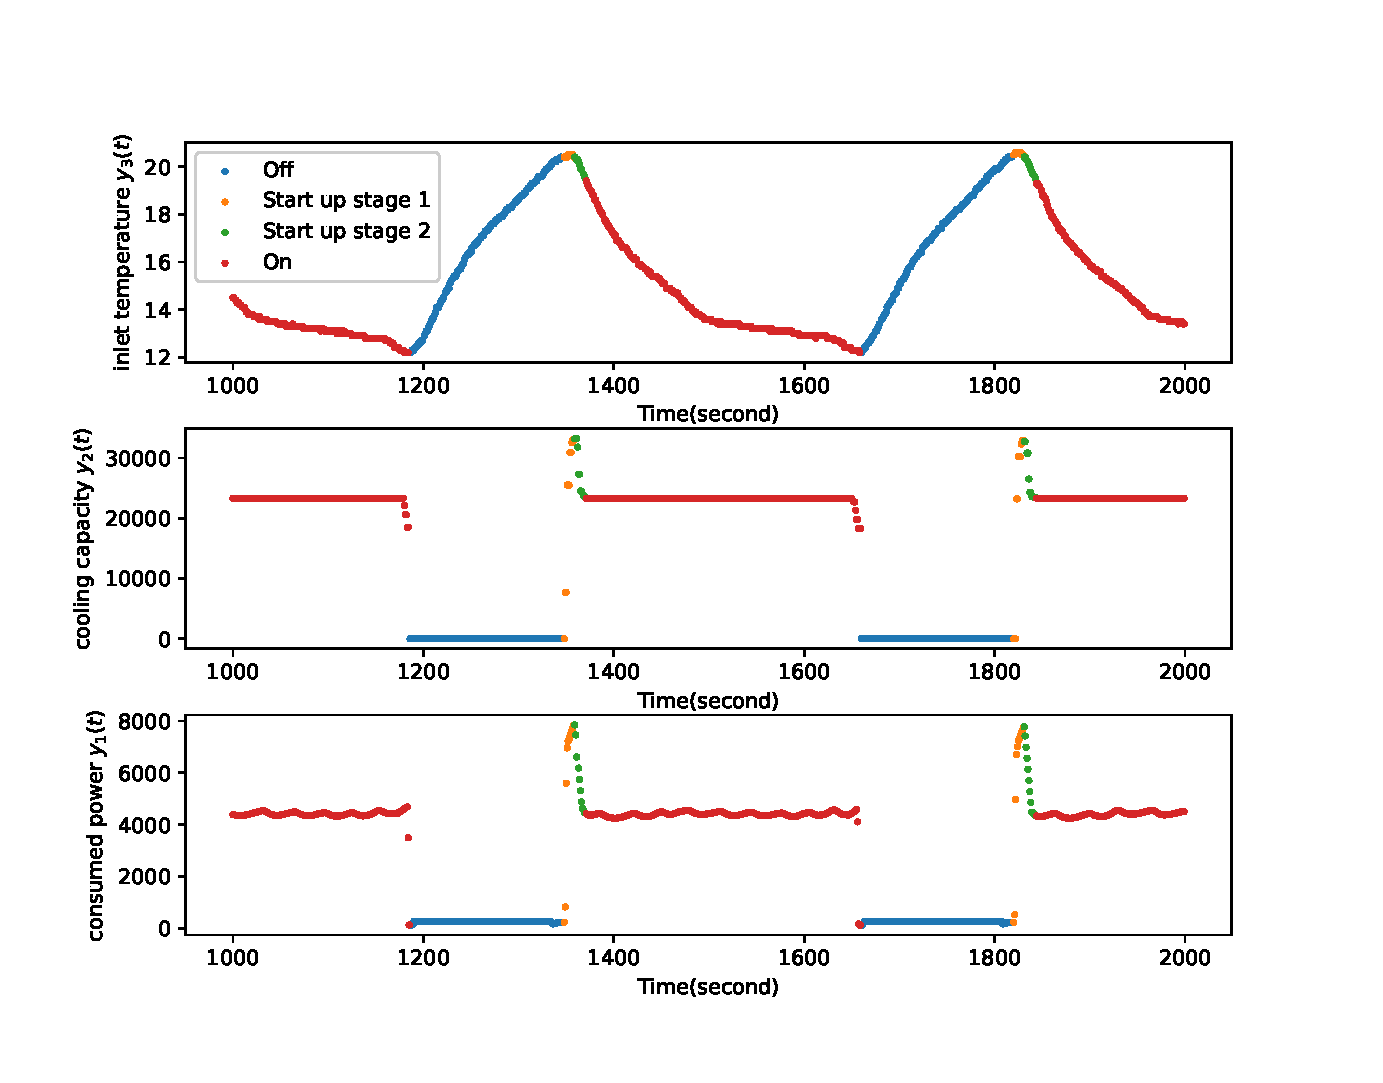
\includegraphics[width=10cm]{figures/chapter4/mark.eps}
%     \caption{Auto Stage labeling result demonstration
%     }
%     \label{fig:stages_mark}
% \end{figure}

% \subsubsection{Multi-stage transformation and duration time prediction}
% According to the prior knowledge, the property of periodic multiple-stage in the system is apparent and we can identify the transform boundaries between adjacent stages from dataset readily.

% The inputs indices include consumed power of the date center $x_1(t)$, room temperature $x_2(t)$. Two inputs variables affect the behaviors of the cooling system and determine three system outputs variables including: instant cooling power $y_1(t)$, cooling production $y_2(t)$, and inlet temperature of cooling system $y_3(t)$.
% Generally, inlet temperature $y_3(t)$ is oscillated periodically in a deterministic range defined by max setpoint $Ti_{max}$ and min setpoint $Ti_{min}$.


% \subsection{Case study 1: Operating Variables Simulation}

\subsection{模型训练}
% \subsection{Model training}
\label{sec:model_training}

本节从Seduce平台采集了四组数据集用于模型的训练与评价,四组数据集均采集于生产运行稳定时段,且运行功率有较大差异,分别为1.7kw,3.8kw,4.2kw,6.3kw。运行功率$x_1(t)$越大,说明当前热负载越高。表\ref{tab:sys_in_out_prior}中汇总了各个数据集的描述、输入输出介绍以及序列长度。在图\ref{fig:state}中,本节统计了不同热负载下,每次\textit{On}阶段和\textit{Off}阶段持续时间的分布情况。
结果表明,阶段持续时间与热负载功率值有较强相关性。在特定的热负载下,阶段持续时间${\tau}_{i}$趋于稳定。
这一结果说明,在开环预测时,利用系统的热负载输入以及外部环境温度动态地预测各个阶段的持续时间以及实现阶段自切换是具有可行性的。
% 与服务器负载功率值有较强相关性,特定数据集下的阶段持续时间分布相对稳定。
% In 图.~\ref{fig:state}, we analyse the statistical properties of duration in each stage. 
% It demonstrates that the distribution of duration ${\tau}_{i}$ is stationary and highly depends on the nearby external inputs.
\begin{figure}
\centering
\hspace{-0.1in}
\subfigure[阶段-\textit{关闭}]{\includegraphics[width=0.45\linewidth]{figures/chapter4/state1.pdf}}\hspace{-0.05in}
\subfigure[阶段-\textit{开机}]{\includegraphics[width=0.45\linewidth]{figures/chapter4/state4.pdf}}
\caption{
% The data of the four data sets are generated at different power of the server, which are 1.7kw, 3.8kw, 4.2kw and 6.3kw respectively. Compare the duration time of system on and off   under different power.
在平均负载不同的四个数据集中,\textit{启动}阶段和\textit{关闭}阶段的持续时间分布箱线图
} %图片标题
\label{fig:state}  %图片交叉引用时的标签
\end{figure}

对于四个数据集,每个数据集中的完整序列长度约为8000-10000,采样时间点为连续非均匀的,平均采样频率约为1条/秒,序列对应的时间长度约为8000s-10000s。
每个数据集的前50\%数据用于模型训练,剩下的数据中,25\%数据用于构建验证集,25\%数据用于模型测试。

对于训练集和验证集,本节使用大小为1600s的滑动窗口对原始序列进行遍历并生成训练样本。
对于每一个训练样本,根据~\ref{sec:4_notations}节的定义,前800s为条件范围,用于编码器求解预测阶段所需的初始状态,后800s为预测范围,模型预测该范围内的系统输出。
在训练过程中,选择验证集中表现最好的模型用于最终的模型评估。
由于系统输入输出的维数较低,且得益于伴随状态法(Adjoint state),不需要存储求解ODE时的完整计算图,训练AJ-ODE-Net网络对于显存的消耗是极低的。因此本节选择了较大的批大小(batch size=4096)以加速训练。
所有数据集的训练样本被随机排序并分批输入到模型训练。训练过程使用了单块型号为NVIDIA TITAN RTX的并行计算设备(GPU),其显存为24G。
隐状态变量$\boldsymbol h(t)$的大小是20,学习率设置为0.005。

% 在测试阶段,没有像构造训练集一样对测试集中的完整序列进行分割。
在测试阶段,未按照构造训练集时采用窗口分割方法对测试集序列进行拆分。
序列的前800s被送入编码器模型以生成初始状态。解码器模块在给定800s之后的剩余序列输入下,以开环的方式预测余下部分的系统输出。预测结果与测试集中的真实输出作对比以评估模型精度。
% During training, the model which performs best in validation dataset will be chosen 
% Owing to low dimensional inputs, we choose a large batch size as 4096 to accelerate training.
% In order to improve the robustness, the training samples of all data sets are randomly ordered and concatenated together before feeding into the model.
% The training phase is executed on a single NVIDIA TITAN RTX with 24G memory.


%when cooling system is off and slower decrease of inlet temperature when cooling system is working.Together with the stages of cooling system, the consumed power of cooling system $y_1(t)$ and cooling capacity $y_2(t)$ also change periodically with the frequencies and phase positions determined by inputs $x_1(t)$ and $x_2(t)$.  


\begin{table}[ht]
    \centering
\caption{系统输入输出, 不同负载下的数据集和模型的操作}
% \caption{System Inputs-Outputs, data sets based on heat load and model options}
\label{tab:sys_in_out_prior}
\begin{tabular}{cll}
\toprule
\multicolumn{1}{c}{}                                  & 变量定义                      & 描述                                    \\ \hline
\multicolumn{1}{c|}{\multirow{2}{*}{输入}}          & \multicolumn{1}{c|}{$x_1(t)$}& 服务器的瞬时功率,  $W$            \\ \cline{2-3} 
\multicolumn{1}{c|}{}                                 & \multicolumn{1}{c|}{$x_2(t)$}& 环境温度, $^{\circ}C$          \\ \hline
\multicolumn{1}{c|}{\multirow{3}{*}{输出}}         & \multicolumn{1}{c|}{$y_1(t)$}& 制冷系统功率,  $W$                  \\ \cline{2-3} 
\multicolumn{1}{c|}{}                                 & \multicolumn{1}{c|}{$y_2(t)$} & 制冷量,  $W$                     \\ \cline{2-3} 
\multicolumn{1}{c|}{}                                 & \multicolumn{1}{c|}{$y_3(t)$}& 入气口温度,  $^{\circ}C$  \\ \hline
\multicolumn{1}{c|}{\multirow{4}{*}{数据集}} & \multicolumn{2}{l}{"1.7k":服务器稳定运行在1.7kw左右, 长度: 8853s}  \\ \cline{2-3} 
\multicolumn{1}{c|}{}                                 & \multicolumn{2}{l}{"3.8k": 服务器稳定运行在3.8kw左右, 长度: 9771s}  \\ \cline{2-3} 
\multicolumn{1}{c|}{}                                 &
\multicolumn{2}{l}{"4.2k": 服务器稳定运行在4.2kw左右, 长度: 8472s}  \\ \cline{2-3} 
\multicolumn{1}{c|}{}                                 &
\multicolumn{2}{l}{"6.3k": 服务器稳定运行在6.3kw左右, 长度: 8418s} \\ \hline
% \multicolumn{1}{c|}{}                                 &
% \multicolumn{2}{l}{Proportion of dataset for training, validation, and test 5:2:5}  \\ \hline
% Dataset split & training: validation:test = 5:2:5 \\ \hline
\end{tabular}
\end{table}

\subsection{应用研究1: 运行变量仿真}
\label{sec:case-study1}
本节使用基于AJ-ODE-Net结构的编码器-解码器框架预测制冷系统的输出。
模型的预测变量为三个:进气口温度、制冷量和制冷机功率。
其中,进气口温度是受制冷系统影响的控制目标变量,表示制冷系统排出的空气温度。制冷量代表制冷系统单位时间产生的制冷量,其直接影响制冷系统中进气口温度的变化~\cite{alonso2020estimating},在压缩机不工作时,制冷量为0。制冷系统开始工作后,制冷量会突然飙升至较高水平。
制冷机功率,表示整个制冷系统的瞬时功耗。在制冷系统工作期间功耗较高,待机期间功耗较低。
% In the first place, the framework is used to simulate the operating variables of the concerned cooling system in real time, three typical variables are selected: inlet temperature, cooling production and cooling power. Where, the first variable inlet temperature is an important thermal target of data center affected by cooling production, indicating the air temperature taken by servers. The second one is cooling production generated by compressor, which acts directly on removing heat during the cooling process~\cite{alonso2020estimating},  compressor consumes most of the electricity in the cooling system. And the third estimated variable is cooling power, indicates the instant power consumed by entire cooling system. 
% 另外,系统运行过程中混合稳定和非稳定的两种过程:当系统产生冷空气时,制冷量和系统功耗可以看作是典型的稳定过程(均值和方差相对稳定)。
% 而在此过程中,进气口温度呈指数型下降,则应视为非稳定过程(均值不断下降)。这种稳定性和非稳定性过程混合的系统在工业系统中很常见,
% 所以有必要将多个H-ODE嵌入到AJ-ODE-Nets模型中。
本节同时引入普通的ODE-Net、ODE-RNN\cite{10.5555/3454287.3454765}、CDE-Net\cite{kidger2020neural}作为本章H-ODE-Net的对比模型。对比模型也可以与本章的阶段转换预测器组合,进而具备跳变系统辨识能力。AJ-ODE-Net与其他模型的对比结果如图\ref{fig:4_models}所示。
% 为了展示H-ODE在多阶段AJ框架中应用的优势,我们对其他可以用来替代H-ODE的模块进行了评估,如嵌入单个ODE模块的结构和嵌入ODE- rnn模块的结构~,并与H-ODE进行了比较,结果如图.~\ref{fig:models}所示。
% In addition, the system operating has a mixture of stationary and non-stationary processes: when the system is producing cold air, energy is consumed stably by compressor, which can be seen as a typical stationary process (with relatively fixed mean and variance). While during this process, the inlet temperature decreases in exponential way, which should be otherwise treated as non-stationary process (the mean keeps dropping). This mixture is commonly seen in industrial systems, and worth the efforts in developing H-ODE network within AJ-ODE-Net module (refer to~\ref{sec:dfa-ode-module}).
% In order to demonstrate the advantages of applying H-ODE in multi-stage AJ framework, other options like one Neural ODE structure and ODE-RNN~\cite{10.5555/3454287.3454765} structure as substitutions for H-ODE are evaluated as well to have a comparison, the results are shown in 图.~\ref{fig:models}.
其中图~\ref{fig:4_models}(a)为真实的系统输出,图~\ref{fig:4_models}(d)为采用带有H-ODE-Net的AJ-ODE-Net模型的预测结果。
在图~\ref{fig:4_models}(b)中,将AJ-ODE-Net替换为一个单一的稳定型ODE-Net,此时各阶段的转换不受持续时间预测器控制。
% 对比(b)和(d)可以发现,使用单一ODE模型难以对各个阶段间的系统切换边界处给出准确的拟合,尤其对于持续时间较短的阶段转换位置,如阶段1与阶段2,预测效果明显差于AJ-ODE-Net。
可以发现,使用单一ODE模型时难以对各个阶段间的系统切换边界处给出准确的拟合,尤其对于持续时间较短的阶段转换位置,如阶段1与阶段2,预测效果明显较差。
在图~\ref{fig:4_models}(c)中,采用ODE-RNN~\cite{10.5555/3454287.3454765}替换了AJ-ODE-Nets中用于建模稳定和非稳定混合输出的H-ODE-Net模块。
可以发现经过替换后,网络难以平滑地预测系统输出。
相比于其他模型,图~\ref{fig:4_models}(d)中AJ-ODE-Net预测的系统输出十分精确,且在阶段转换的边界处能够极好地识别系统输出的剧烈变化。
% Where 图.~\ref{fig:models}(a) is the pattern of original data sets and 图.~\ref{fig:models}(d) is the estimation results by adopting AJ-ODE module with H-ODE-Net cells. 
% In 图.~\ref{fig:models}(b), the AJ-ODEs module is replaced by one stationary neural-ODE, in this case, transition of stage is not governed by duration predictor, which could have troubles in precisely fitting dynamics of each stage, especially for the short stage transitions. In 图.~\ref{fig:models}(c) the hybrid stationary and non-stationary 
% H-ODE cells in AJ-ODE-Nets are replaced by another widely used structure ODE-RNN~\cite{10.5555/3454287.3454765}, which can hardly simulate smooth physical process. 
\begin{figure*}
\centering
\hspace{-0.2in}
\subfigure[原始数据]{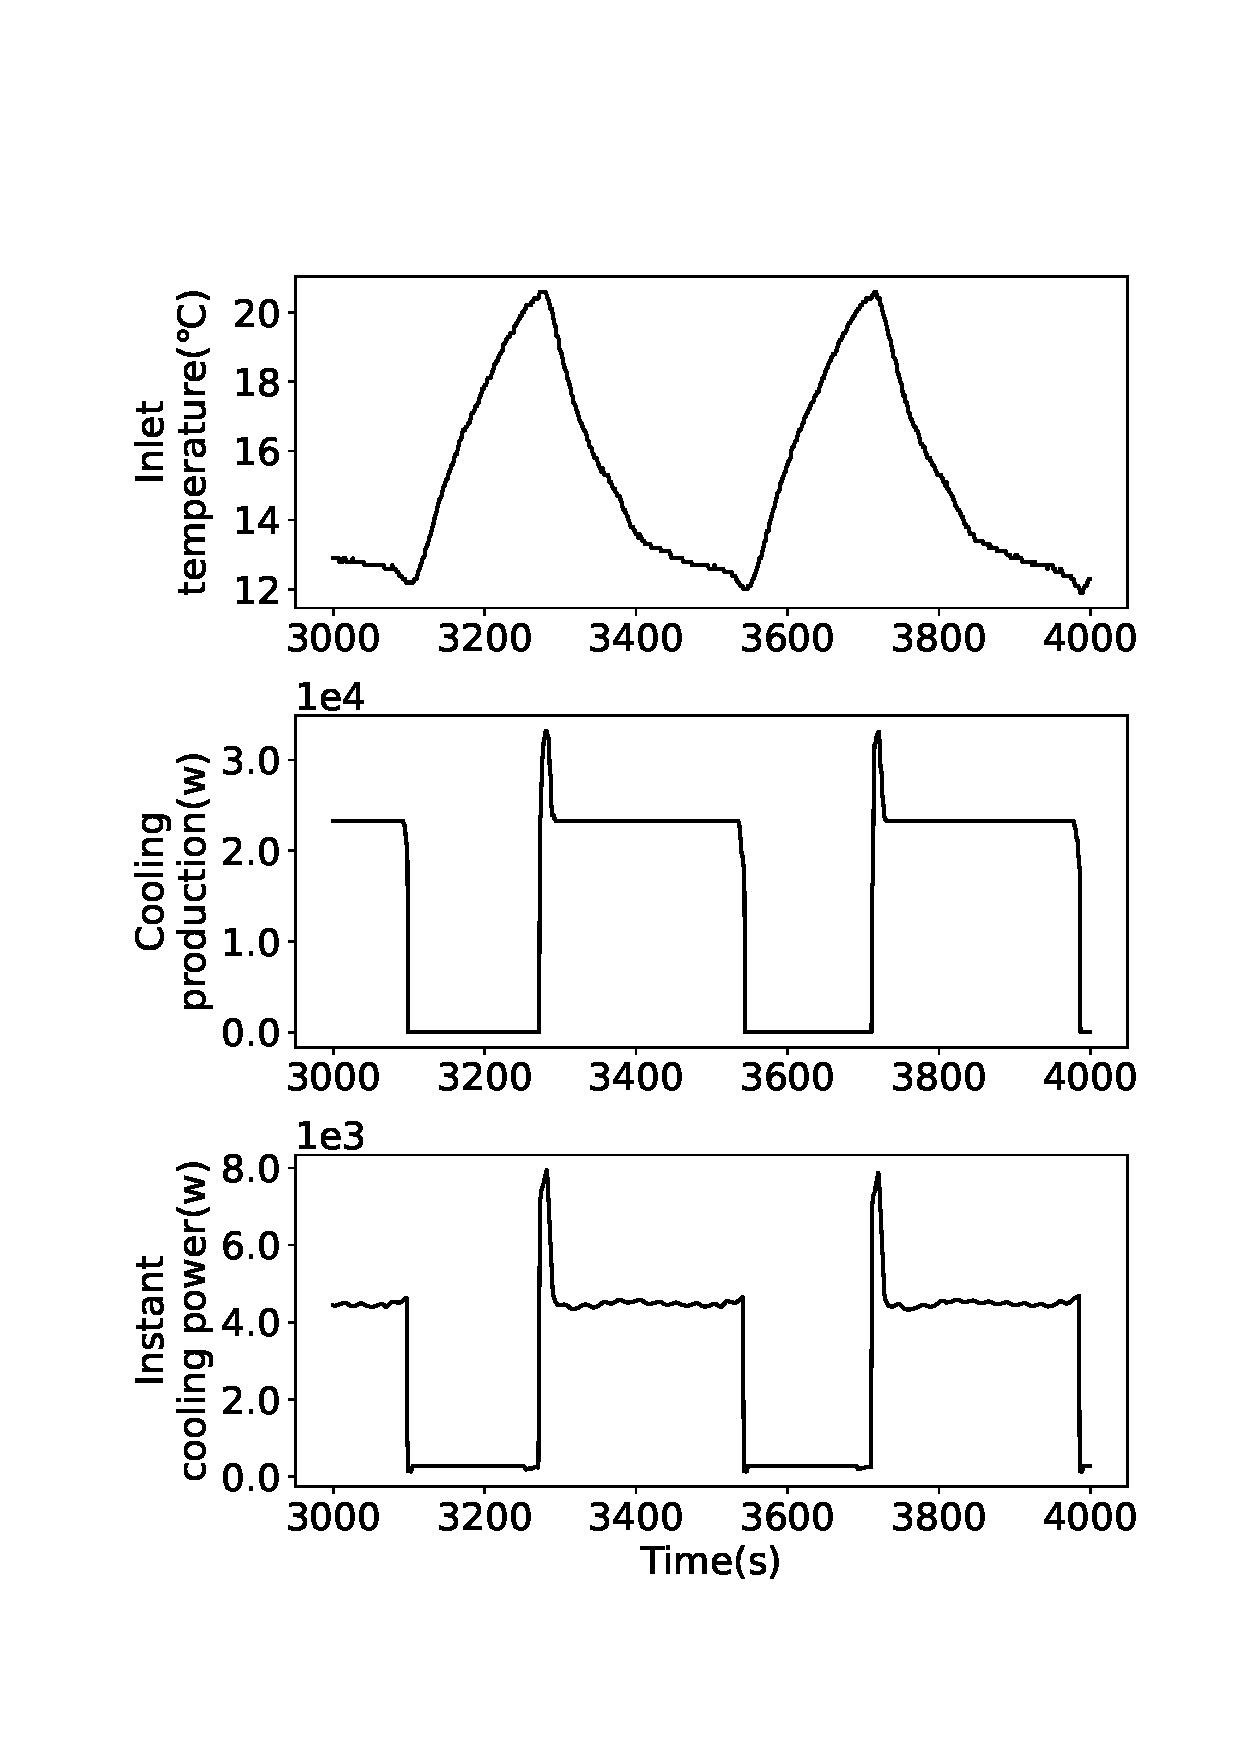
\includegraphics[width=0.45\linewidth]{figures/chapter4/truth.pdf}}\hspace{-0.08in}
\subfigure[单ODE网络]{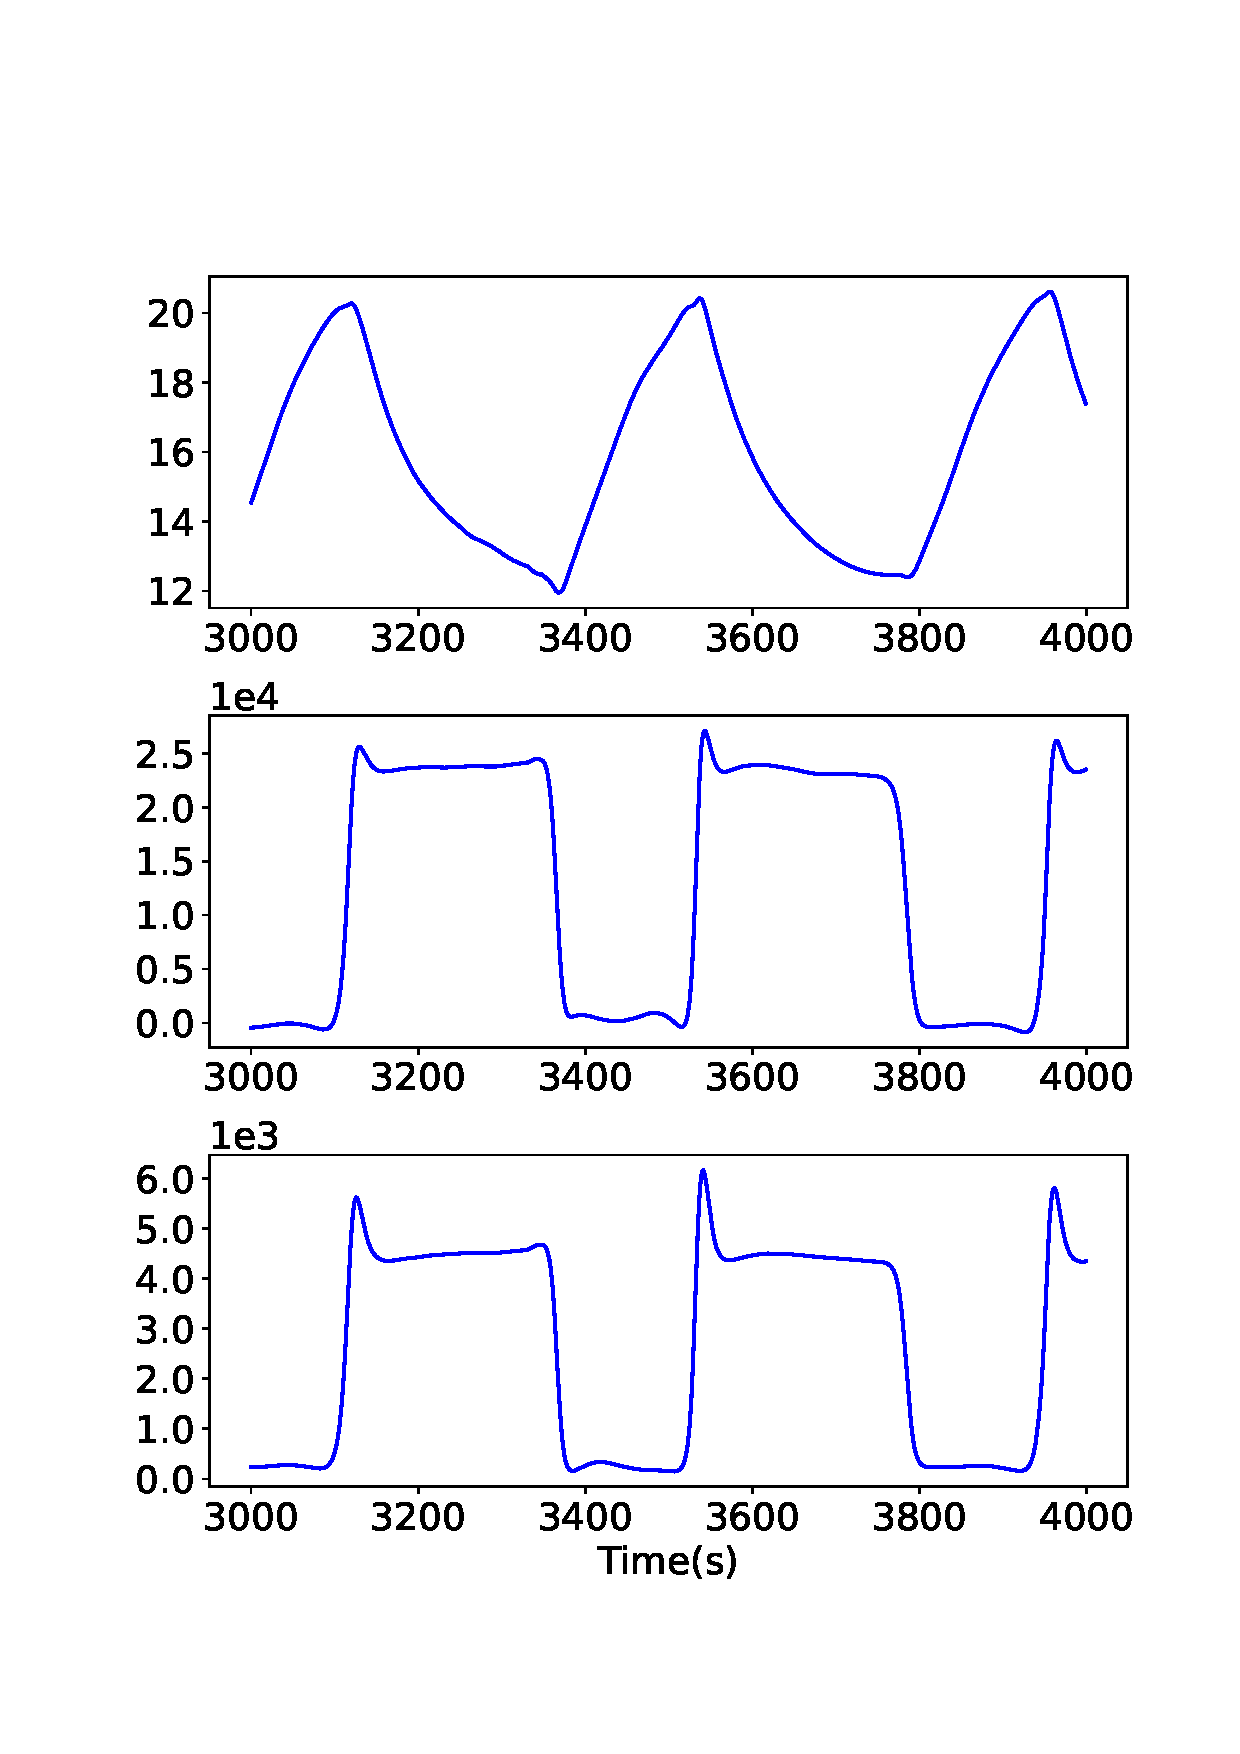
\includegraphics[width=0.45\linewidth]{figures/chapter4/one.pdf}}\hspace{-0.08in}
\subfigure[自跳跃结构+ODE-RNN]{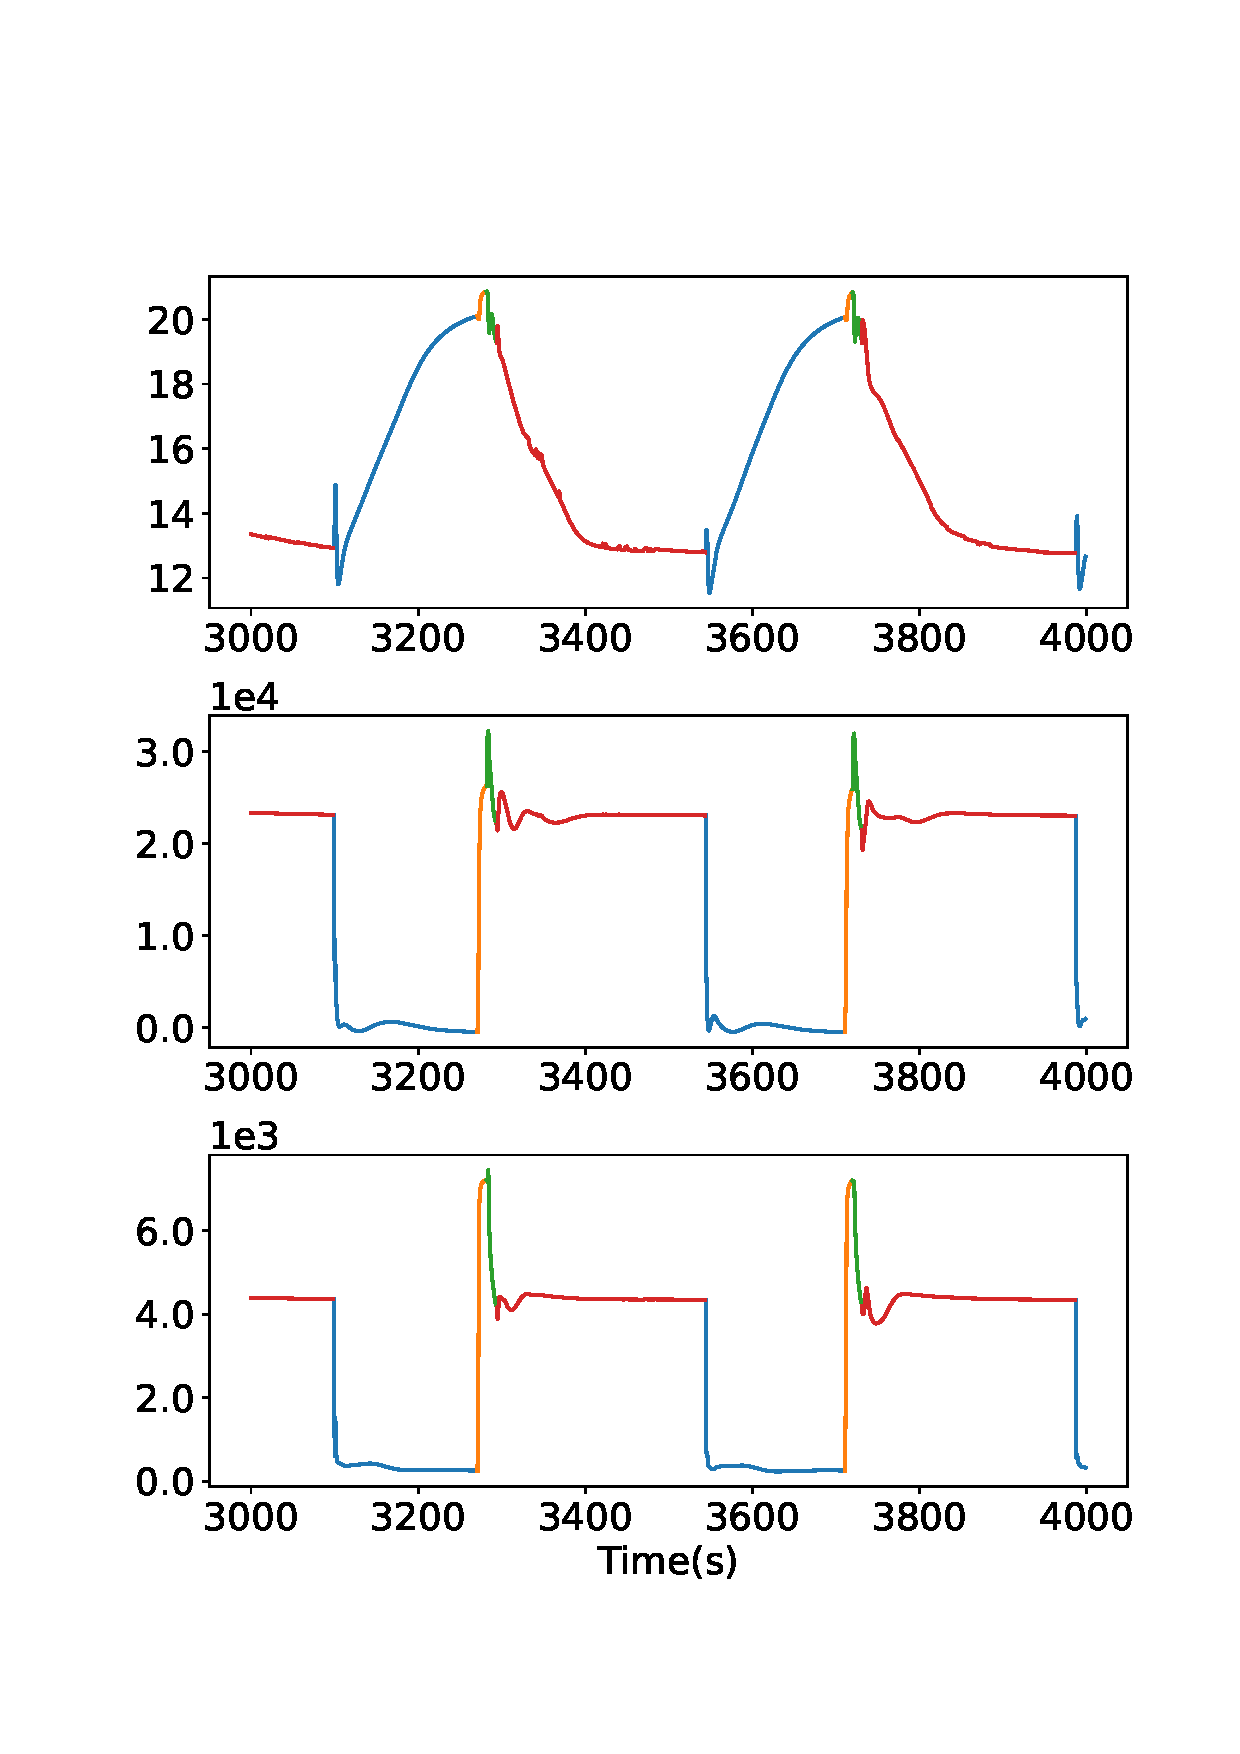
\includegraphics[width=0.45\linewidth]{figures/chapter4/rnn.pdf}}\hspace{-0.08in}
\subfigure[自跳跃结构+H-ODE-Net(本文方法)]{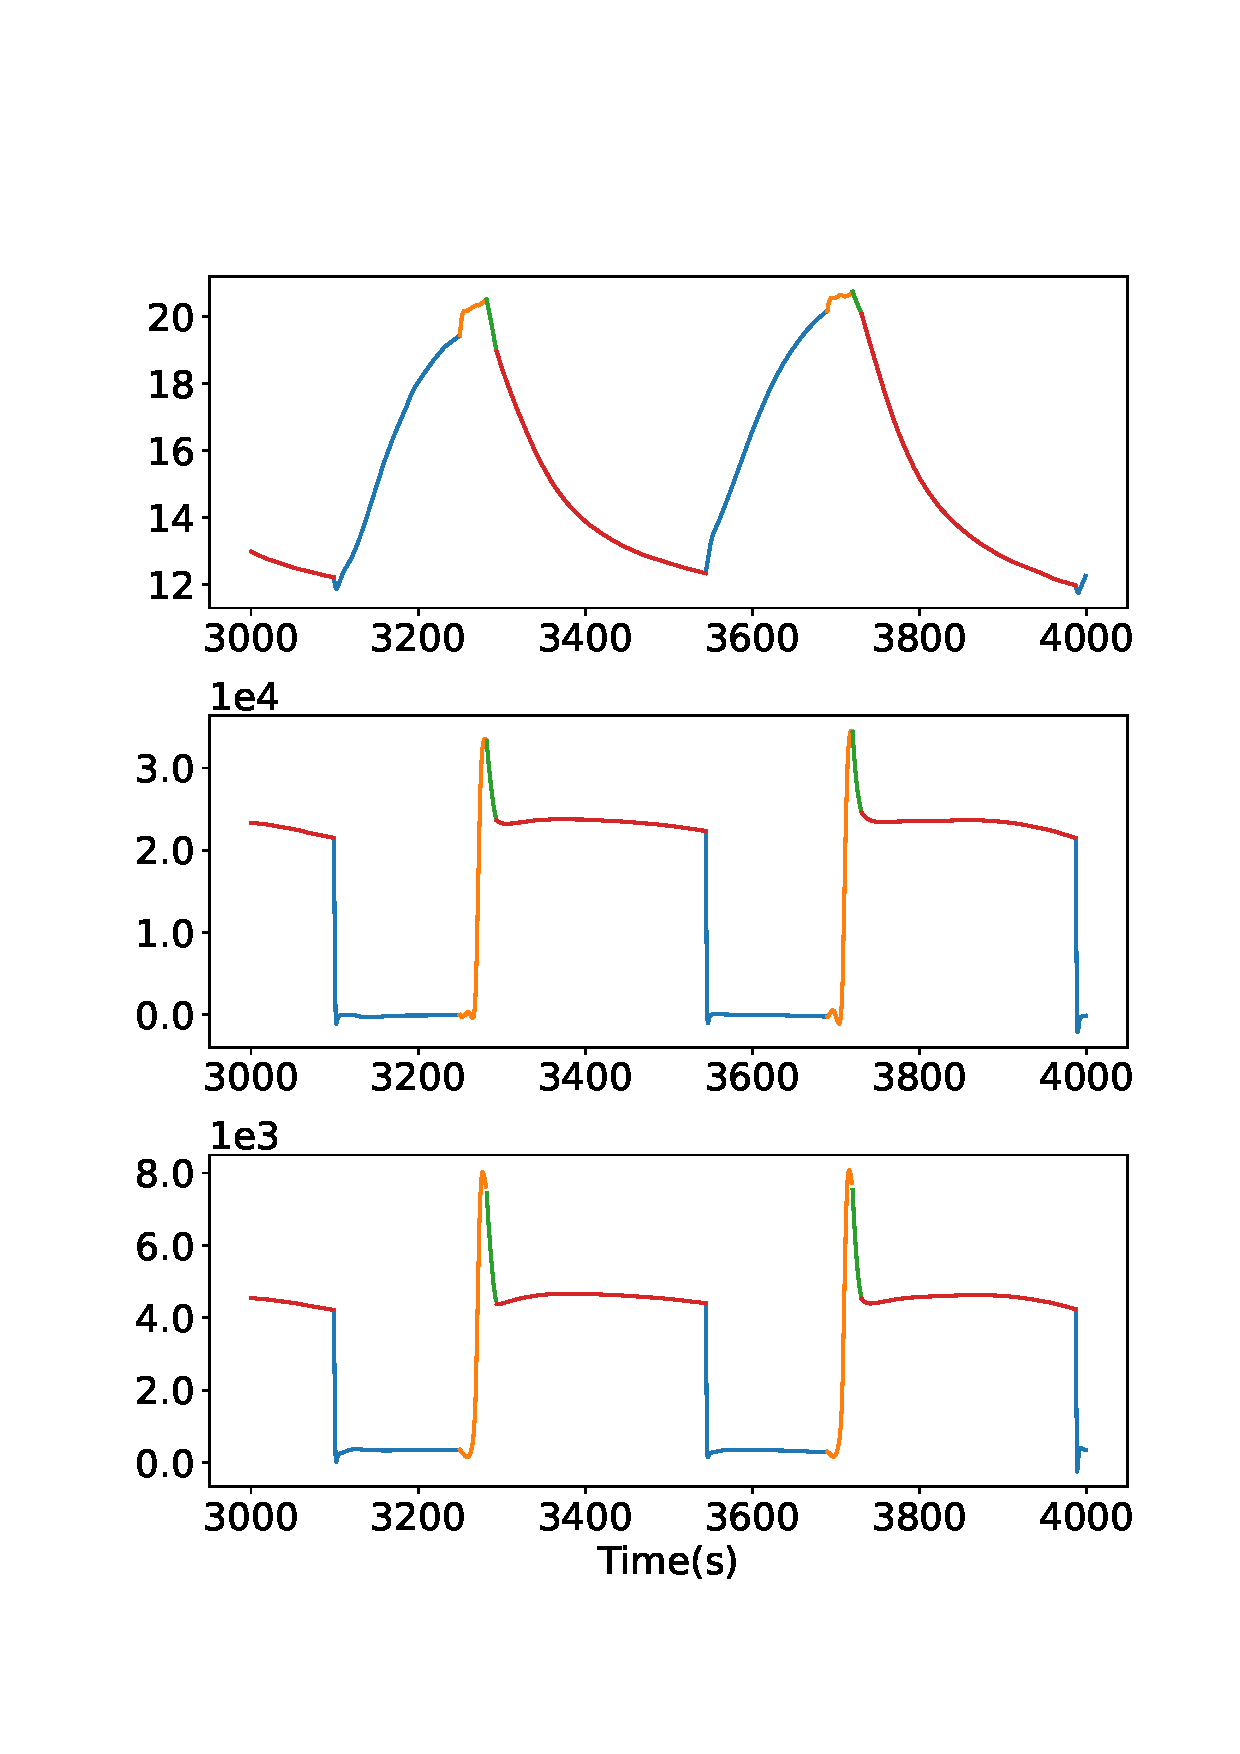
\includegraphics[width=0.45\linewidth]{figures/chapter4/ours.pdf}}
\caption{不同模型预测进气口温度、制冷量、制冷机功率的效果对比} %图片标题
\label{fig:4_models}  %图片交叉引用时的标签
\end{figure*}
% 图.~\ref{fig:}
% \centering
% \hspace{-0.1in}
% \begin{figure}
%     \centering
%     \hspace{-0.1in}
%     \subfigure[The time of state-off]{\includegraphics[width=4.7cm]{figures/chapter4/3.8k.png}}\hspace{-0.2in}
%     \subfigure[6.3k]{\includegraphics[width=4.7cm]{figures/chapter4/6.3k.png}}
%     \includegraphics[width=10cm]{figures/chapter4/3.8k.png}
%     \caption{Prediction results of 3.8k-power}
%     \label{fig:3.8k-power}
% \end{figure}
% \begin{figure}
%     \centering
%     \includegraphics[width=10cm]{figures/chapter4/6.3k.png}
%     \caption{Prediction results of 6.3k-power}
%     \label{fig:6.3k-power}
% \end{figure}
上述实验表明,使用多阶段模型能够将先验知识集成到模型中,相比于单模型结构,能够更好地预测多阶段系统的阶段转换边界。
同时,结合了非稳定输出和稳定输出的H-ODE-Net模型能够有效地对系统的多个输出项进行学习,相比于忽视了系统输出时序特性的ODE-RNN模型,能够更准确地预测系统的输出。

% In addition to the predicted accuracy, in using AJ method, the prior knowledge can be integrated into models, to enable advanced studies like the simulation of configuration adjustments, dynamical control and energy consumption optimization. Conversely, for one Neural-ODE or AJ-ODE-RNN structures, it is not applicable.
接下来,本小节将定量地评估不同模型的预测精度。由于本文关注于开环预测问题并且需要模型自发地进行阶段切换。伴随着预测范围长度的增加,对于相位的估计误差也将不断累积。
当预测结果中各阶段开始、结束的位置与系统真实输出中阶段的起止位置无法对齐时,此时点对点的误差评估并不适用于量化评估模型的预测误差。
因此,本节对模型预测功耗的长期累积结果进行评估。
对于不同功率的数据集,采用训练过的模型预测制冷系统在未来预测范围$[{t_I:t_{I+L}}]$(共120分钟)下的功耗。
% In terms of the estimation accuracy, given that AJ-ODE-Nets is applied for open loop estimation and govern the stage transition automatically, the running phases could be affected significantly by the initial point and accumulative error, therefore the point to point accuracy is less meaningful. 
% Accordingly, in order to evaluate the long term simulation capability of the framework, the accumulative energy consumption is estimated over different predictive length, from five minutes to two hours. 
% For the datasets with different power, we employ the trained model to predict the future energy consumption with the predictive range $[{t_I:t_{I+L}}]$ equaling 120 minutes.
% The length of the predicted range ${t_I:t_{I+L}}$ is 120 minutes.
% The predictive error of the accumulative power consumption is evaluated sectionally and measured as Mean Absolute Percentage Error (MAPE).
% By defining the size of the evaluation window as $T$, the prediction error of consumed power, $E(T)$, is measured as:
在序列预测结果基础上,按时间尺度对瞬时功耗进行积分以得到某一时间长度(T)下的累积功耗预测值。
进一步地,可以定义预测功耗的平均绝对百分比误差,$\text{MAPE}(T)$:
% The Mean Absolute Percentage Error (MAPE) of the predicted energy consumption, $\text{MAPE}(T)$, is defined based on the size of the evaluation window $T$:
% \vspace{-5pt}
\begin{equation}
\text{MAPE}(T) = \frac{100\%}{n}\sum\limits_{i=1}^{\lfloor\frac{t_{I+L}-t_I}{T}\rfloor}\text{APE}(t_I+T*(i-1),t_I+T*i)
\label{equ:energy_mape}
\end{equation}
其中,其中绝对百分比误差(APE)定义如下:
\begin{equation}
\text{APE}(t_1,t_2) = \left|\frac{\int_{t_1}^{t_2}\hat{y}_1(t)dt-\int_{t_1}^{t_2}y_1(t)dt}{\int_{t_1}^{t_2}y_1(t)dt}\right|
\end{equation}
其中,绝对百分比误差$\text{APE}(t_1,t_2)$衡量了时间范围$[t_1, t_2]$内预测功耗和真实功耗之间的相对误差。
图\ref{fig:mape_evolution}描述了评估窗口的大小T对于评估结果$MAPE(T)$的影响。
可以看出,随着$T$的增加,$\text{MAPE}(T)$ 在开始时剧烈下降,然后缓慢下降。
当评窗口大小超过35分钟时,所有数据集的MAPE都趋于稳定,说明此时真实输出序列与预测序列之间的阶段起止位置相位差对于评估长期功耗的预测精度不再产生影响。
因次本节对比了$T=30$分钟下,不同模型对于累积功耗预测结果的MAPE,结果如表~\ref{tab:Compare power}所示。
对于所有数据集,AJ-ODE-Net预测结果的MAPE稳定低于5\%,优于其他三个对比模型。
充分证明了本文提出的AJ-ODE-Net模型及编码器解码器框架能够以开环预测的方式在长时间尺度下精确地仿真制冷系统的累积功耗。

从计算复杂性的角度,本节对四个模型在测试集单批数据上执行式\eqref{equa:initial_state}以及式\eqref{equ:decoding}两个过程的时间消耗进行了对比。
普通ODE-Net作为耗时最短的模型,将其时间消耗作为基准,其他模型的推理时间均除以该基准以得到相对尺度下的耗时指标。
相应地,普通ODE-Net的相对时间消耗为1.0。对比结果如表\ref{tab:Compare power}的最后一列所示。
相对时间尺度下的对比结果表明引入阶段转换预测器会增加计算开销,该时间消耗主要用于更新阶段变量及阶段持续时间。

% % The Mean Absolute Percentage Error (MAPE, see 式~\ref{equa:mape}) has been calculated between real and estimated energy consumption in the test datasets. We select a series with a time duration of 120min, In order to calculate the power consumption of different duration $t_r$, from 5 minututes to 120 minututes.According to the formula $ n=120/tr$, get n sample points. 
% % Where, $n$ is the number of sample points, $\hat{e}_i$ is the estimated value and $e_i$ is the real value.  
% % As illustrated by 式~\ref{equa:energy},  where the value $a$ is the beginning of this sequence time, the value $b$ is the ending, and $y_1(t)$ is the instantaneous consumed power of the cooling  system. 
% % The energy consumption is calculated through the integral of power over a period of time. 
% where absolute percentage error(APE) measures the relative error of the estimated energy consumption, which is calculated through the integral of power over a period of time $[t_1, t_2]$. 
% 图.~\ref{fig:mape_evolution} describes how does the size of evaluation window affect the evaluated results $E(T)$.
% % The 图.~\ref{fig:mape_evolution} shows the MAPE of the energy consumption estimation results over prediction duration. 
% It can be seen that, with the increase of $T$, $\text{MAPE}(T)$ declines dramatically at the beginning then becomes smaller and smaller. 
% When the size of evaluation window exceeds 35 minutes, the MAPE of all datasets are stably below 5\%, the phase difference will have little impact on estimating long-term energy consumption. 
% Tab.~\ref{tab:Compare power} also compares the MAPE of predicted energy consumption from proposed AJ-ODE-Net with the results from the other competitors.
% The results indicate that, in terms of the open loop estimation, the proposed framework can eliminate the impact of initial point and obtain satisfying accuracy for energy consumption simulation with a predictive range longer than half an hour. 
\begin{table}[t]
    \centering
    % \caption{
    % of H-ODE-Net and 
    % Power estimation error comparison between One-ODE and H-ODE ,The total length of each test set is 120 minutes. Select the sequence every 30 minutes, calculate the power consumption of the truth value and the predicted value, and then calculate the MAPE. Truth power consumption$P_{truth}=(p_1,p_2,p_3,p_4)$,Predicted power consumption$P_{pred}=(\hat{p_1},\hat{p_2},\hat{p_3},\hat{p_4})$
    % The comparison of energy consumption prediction and the relative computational efficiency}
    \caption{不同模型累积能耗预测精度和推理时间的对比}
    % \resizebox{0.9\linewidth}{!}{
    \begin{tabular}{lccccc} 
    \toprule
                                & \multicolumn{4}{c}{\textbf{\textbf{热负载}}} & \multirow{2}{*}{\begin{tabular}[c]{@{}c@{}}相对 \\时间\end{tabular}}  \\
    \multicolumn{1}{c}{}        & 1.7k          & 3.8k          & 4.2k          & 6.3k               &                                                                           \\ 
    \hline
    \textbf{AJ-ODE-Net}(本文模型) & \textbf{4.20} & \textbf{1.51} & \textbf{3.46} & \textbf{2.53}      & 3.2                                                                        \\
    单个ODE-Net              & 6.18          & 19.99         & 6.24          & 3.39               & 1.0                                                                         \\
    自跳跃结构+受控微分方程网络\cite{kidger2020neural}     & 8.25         & 2.73          & 6.62         & 3.87              & 3.8                                                                        \\
    自跳跃结构+ODE-RNN & 38.26         & 9.94          & 10.58         & 31.90              & 3.4                                                                        \\
    \bottomrule
    \end{tabular}
    % }
    \label{tab:Compare power}
    % \vspace{-15pt}
    \end{table}

% \begin{equation}
% \label{equa:mape}
%     MAPE=\frac{100\%}{n}\sum\limits_{i=1}^{n}|\frac{\hat{e_i}-{e_i}}{e_i}|
% \end{equation}


% \begin{equation}
% \label{equa:energy}
%     Energy = \int_{a}^{b}y_1(t)dt
% \end{equation}

% \begin{equation}
% \label{equa:energy}
%     n = 2/x
% \end{equation}

\begin{figure}
    \centering
    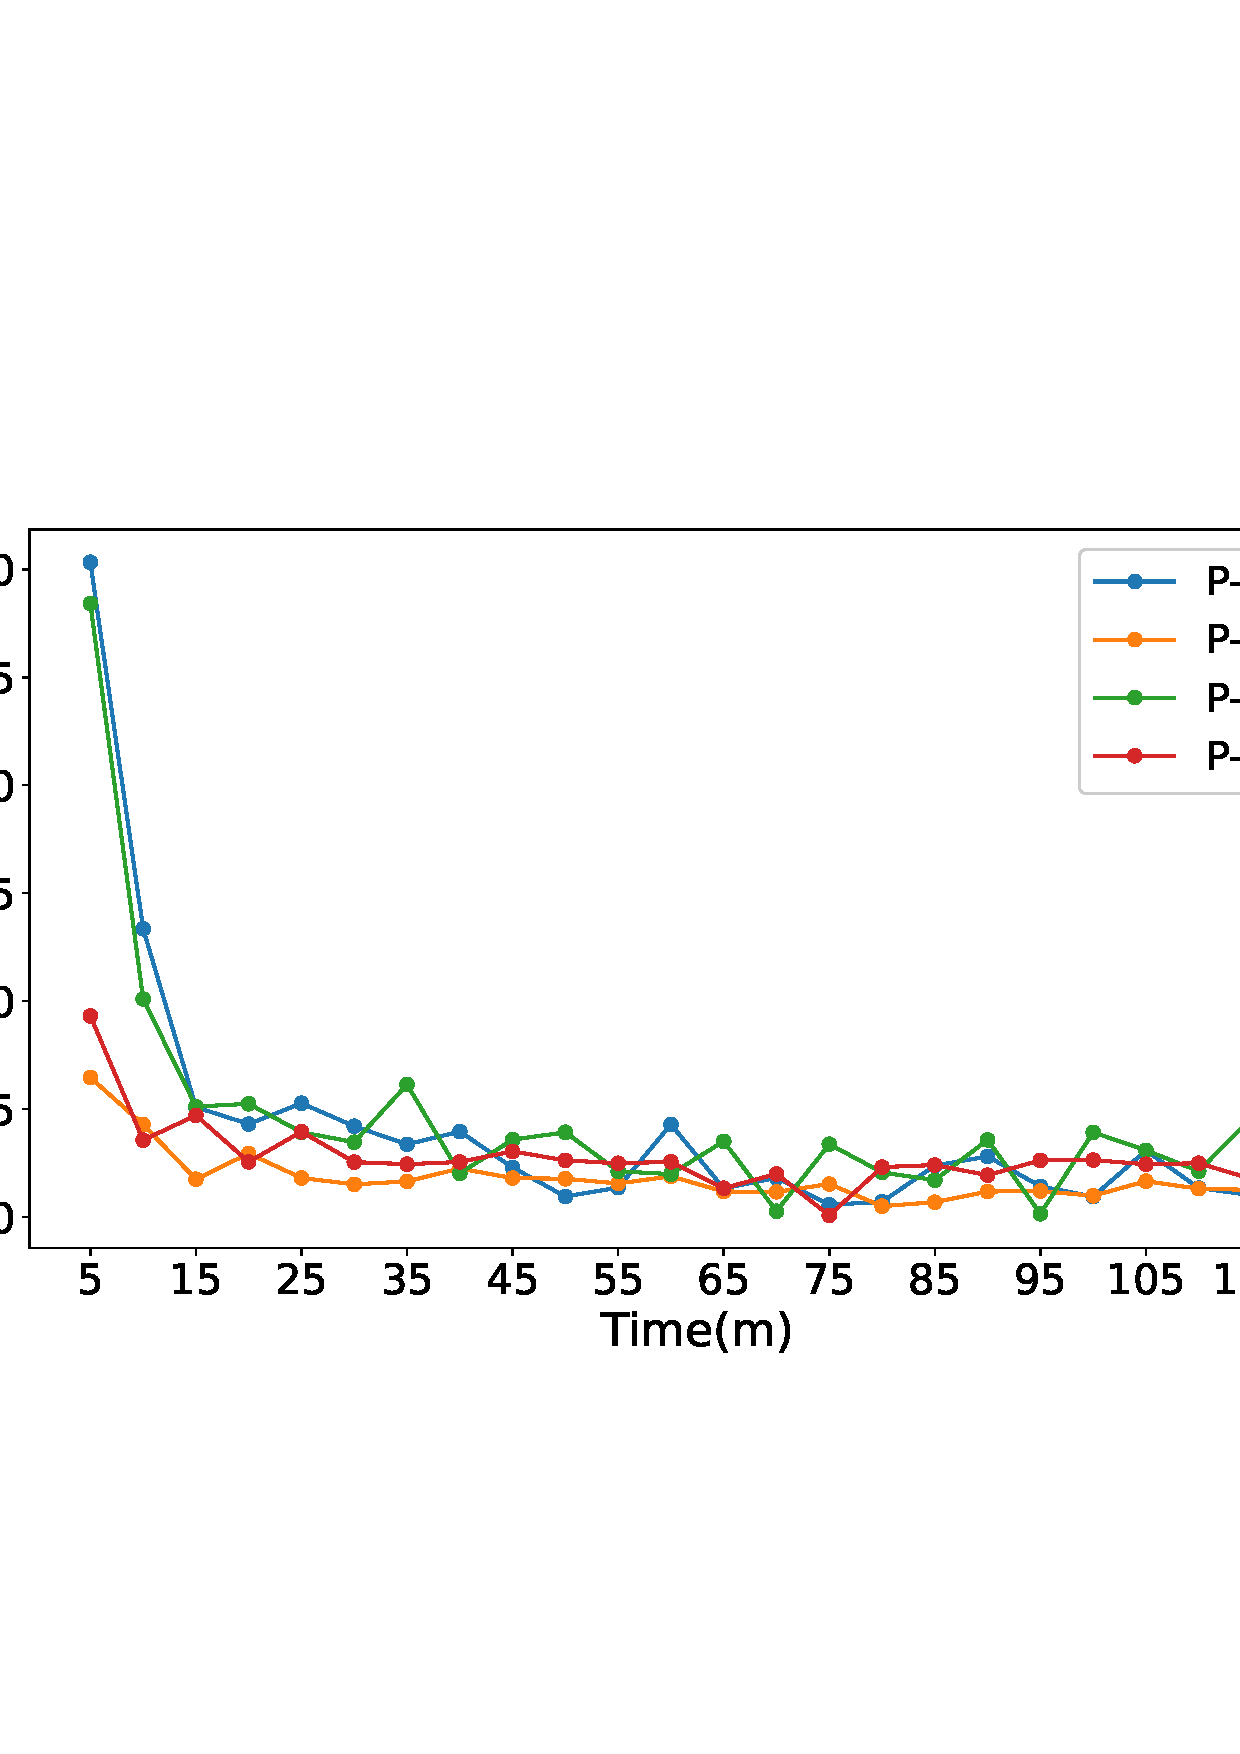
\includegraphics[width=0.8\linewidth]{figures/chapter4/power_error.pdf}
    \caption{预测不同时间长度的功耗的MAPE的变化}
    \label{fig:mape_evolution}
\end{figure}

%Relative error of predicted power consumption at different intervals,According to the instant cooling power sequence value predicted by AJ-ODE-Nets, calculate the power consumption of the system over a period of time, compare it with the real power consumption value, and calculate the error.  Compare the power consumption error between the real value and the predicted value for different duration time (5min, 10min... 120min)


%Compare the prediction effects of different models. 图.re a is the truth sequential data, figure B is the prediction result of one stable ODE model, figure C is the experimental effect of Ode RNN, and figure D is the result of our model

\subsection{应用研究2: 制冷系统进气口温度设定点优化}
\label{sub:case-study2}
进气口温度上下限设定值(上限$Ti_{\max}$和下限$Ti_{\min}$)是影响制冷系统运行、保证运行环境安全的关键设置参数。
% 通常,系统要设定通入进气口的空气温度阈值,以保证运行环境的安全。
% 通常,对于大部分的制冷系统,初始的进气口温度设定点是固定的,配置值低于ASHRAE TC9.9~\cite{ashraeTC992011}(数据中心电源设备热指南和最佳实践)中定义的标准,没有充分考虑实际的制冷需求。
对于本章研究的制冷系统,其默认温度阈值为$12^\circ C$,$20^\circ C$。
从数据集可以观察到进气温度在上下阈值之间周期性变化。
由于默认温度设置未充分考虑实际的制冷需求,会存在一定程度的能源浪费。
出于提高能源效率以及确保生产过程安全的目的,本节在保持温度上阈值不变的情况下,通过优化下阈值以减少制冷消耗。
然而,想要精确地找到最佳温度阈值是困难的。
如果阈值设置太低,由于过度制冷会浪费大量电能。
如果阈值设置太高,压缩机的制冷重启过程将更加频繁。
从图~\ref{fig:4_models}中可以看出,制冷系统重新启动时的功耗显著高于提供稳定制冷时的功耗。
因此,盲目地增加温度下阈值反而可能会导致整体能耗的增加。
% 实际上,最佳温度设定点随热负载的不同而变化,尤其是温度下限。如果下限设置过低,会因过度制冷过多而浪费电能;过高会导致压缩机频繁停机和启动,如图1所示(见表~\ref{tab:cooling_dfa}),在阶段一启动时功率峰值会很高,这些峰值过多会浪费额外的电能,。

本节试图寻找最优温度下限以期望达到最佳的能源效率。形式化地,寻找最优温度下限$Ti_{\min}^{*}$可以表示为一单目标优化问题,问题中需要考虑的因素包括:热负载、环境温度、进气口温度的上下限:
\begin{equation}
    \begin{aligned}
       Ti^*_{\min}&=\mathop{\arg\min}\limits_{Ti_{\min}} \int_{0}^{T} \hat{y}_{1}(t) dt \\
       &\text{s.t. } \hat{\boldsymbol{Y}}_{0: T}=F\left(\boldsymbol{X}_{0: T},Ti_{\min}, Ti_{\max},\boldsymbol{\zeta}\right),
       Ti^*_{\min}\leq \hat{y}_{3}(t) \leq Ti^*_{\max}
    %    &\text{s.t. }\begin{aligned}
    %    \end{aligned}
    %    \text{s.t. } \hat{\boldsymbol{Y}}_{0: T}=F\left(\boldsymbol{X}_{0: T},Ti_{\min}, Ti_{\max},\boldsymbol{\zeta}\right)
    %    &\text{s.t. } \hat{\boldsymbol{Y}}_{0: T}=F\left(\boldsymbol{X}_{0: T},Ti_{\min}, Ti_{\max},\boldsymbol{\zeta}\right)
    \end{aligned}
    \label{equ:optimazition}
    \end{equation}
其中$\hat{\boldsymbol{Y}}_{0: T}$和$\hat{y}_{1}(t)$分别表示模型预测的系统输出以及预测出的瞬时功耗。
在给定系统输入和恒定上限值的条件下,被优化变量为温度下阈值,优化目标是最小化累计能耗。
式\eqref{equ:optimazition}中的$\boldsymbol{X}_{0: T}$为测试数据集中的系统输入,其中包括所有时刻的热负载以及环境温度。
$F(\cdot)$表示在给定输入和温度阈值$Ti_{\max}$和$Ti_{\min}$下,预测制冷系统的输出。
% The inlet temperature set points are one of the key configurations of cooling systems. Generally, they put the temperature variation thresholds (upper and lower boundaries) for the air temperature to the front of the servers, to guarantee the ambient and secure operating environment. 
% Normally, for the workplace like Data Centers, the initial set points are fixed and configured far below the standards defined by ASHRAE TC9.9~\cite{ashraeTC992011} (Data Center Power Equipment Thermal Guidelines and Best Practices), without considering the actual cooling requirement. 
% Actually, optimal temperature set points vary with the heat load, especially for the lower boundary: if it is set too low, energy will be wasted due to over cooling; if too high, compressor may suffer from frequent stop and restart, additional energy can be wasted due to too many power peak as seen in stage 1 (refers to Tab.~\ref{tab:cooling_dfa}). 

本节利用上一节~\ref{sec:case-study1}中训练的编码器-解码器AJ-ODE-Net模型,
在给定不同下阈值温度设定点的情况下,仿真制冷系统能耗以及进气温度变化,同时统计120分钟内的累积制冷能耗。
实验采用\secref{sec:case-study1}中热负载分别为1.7k、3.8k和6.3k的三个数据集。
温度下阈值设置点从$12^{\circ}C$逐渐增加到$18^{\circ}C$,调整间隔为$0.5^{\circ}C$ 。
% In order to simulate the cooling system with different $Ti_{\min}$, the prediction in $F(\cdot)$ is slightly different from the trained model $f(\cdot)$.

为了模拟不同$Ti_{\min}$下冷却系统的运行过程,$F(\cdot)$中的预测过程与式\ref{equa:problematique}的原始训练模型$f(\cdot)$略有不同。
% In particular, the sojourn time predictor in stage \textit{On} is replaced by a specific transformation rule.
在阶段\textit{On}下的持续时间预测器被特定的转换规则所替代。
% Just as the rule in Table~\ref{tab:cooling_dfa}), the stage immediately transitions from 3 (\textit{On}) to 0 (\textit{Off}) if the inlet temperature is cooled down to $Ti_{\min}$. 
如表~\ref{tab:cooling_dfa}所示规则,当进气口温度经过冷却下降到$Ti_{\min}$,预测模型立即将阶段变量从3(\textit{On})过渡到0(\textit{Off})。
    % The stage transition predictor in the proposed model is designed based on sojourn time prediction,  nevertheless, the rules could also be set manually in order to meet simulation requests.
尽管AJ-ODE-Net中的阶段转换预测器是基于持续时间预测器设计的,为了满足不同制冷运行参数仿真的需要,模型支持将持续时间预测器替换为其他的状态转换规则。
虽然在上述模拟过程中的温度下限与训练数据集对应的阈值参数是不同的,但AJ-ODE-Net允许手动调整阶段过渡阈值以支持外推预测。
    % Although the lower temperature threshold in simulations is out of the range of the training dataset, AJ-ODE-Net can still support extrapolation by adjusting manually stage transition thresholds.
相比于没有引入系统先验的稳态模型~\cite{Yilmaz2007},基于先验知识设计的模型具有更好的可扩展性,更便于实现灵活的系统仿真。
    % Compared with the steady state model~\cite{Yilmaz2007}, the prior knowledge-informed model is more interpretable and extensible.
    % Meanwhile, in order to model the variation of inlet temperature as a non-stationary process, the temperature is made to climb steadily during stage \textit{Off} and decreased steadily during stage \textit{On}.
同时,本章将进气口温度的变化建模成非平稳过程,使得在阶段\textit{Off}期间,进气温度将会稳定地上升,在阶段\textit{On}期间,温度会稳定地下降。
% 这两个性质能够确保进气温度必然能够触达给定的阈值。
    % This property is consistent with the prior knowledge of the system and is necessary to guarantee that the inlet temperature will continue to vary until reach the wanted thresholds.
这一特性与系统的先验知识一致,是保证进气口温度能够持续变化直至达到阈值的必要条件,有效避免了模型无限期停留某一阶段内难以跳出的情况。

% 在下边界温度设定点不同的情况进行系统仿真实验中,我们对于从\textit{On}阶段到\textit{Off}阶段的转换过程,用了一个转换规则替换了持续时间预测器。
% 如表~\ref{tab:cooling_dfa}所示的系统先验知识,随着制冷系统温度降低,当前进气口温度小于$Ti_{min}$时,系统将切换到阶段 \textit{Off},
图~\ref{fig:lowerbound_simulation}展示了对于热负载约为3.8k的数据集,设置不同进气温度下限时,制冷系统在1000秒内的瞬时功率变化情况。
% 对制冷系统的影响。
% 仿真时间为1000秒。
随着温度下限设定点从$12^{\circ}C$增加到$18^{\circ}C$,在相同的持续时间内,系统处于稳定制冷阶段的时间不断缩减。与此同时,1000秒内包含了更多的制冷系统启停周期。这导致系统的主要功耗来自于由\textit{Off}阶段转变为\textit{on}阶段的系统启动功耗,而非制冷功耗。

% In order to find the optimal lower boundary temperature set points under different heat loads. 
% we make use of the Encoder-Decoder AJ-ODE-Net model built in the first case study~\ref{sec:case-study1}, and run simulations by calculating the energy consumption within same duration under different lower temperature set point for three datasets.
% % as they represent for different heat loads (higher IT loads will generate more heat). 
% The three datasets represent for different average heat loads (higher IT loads will generate more heat) including 1.7k, 3.8k, and 6.3k.
% In each simulation with specific lower boundary temperature $Ti_{min}$, we substituted the duration predictor with a rule in the transformation from \textit{On} stage to \textit{Off} stage.
% With the cooling system brings the temperature down, the system will switch to the stage \textit{Off} when the current inlet temperature is smaller than $Ti_{min}$, as like the system prior knowledge shown in Tab.~\ref{tab:cooling_dfa}.
% % The set points can be modified in Stage Transition Predictor (refers to Sec.~\ref{sec:stage_trans_predic}), where the configurations are integrated as system prior knowledge. 
% 图.~\ref{fig:lowerbound_simulation} illustrates the impact of different lower boundaries on the behaviors of cooling system (dataset 3.8k), with the set point increasing from $12^{\circ}C$ to $18^{\circ}C$, more loops are included within same duration.
% The main stages which consume the energy most change from \textit{On} stage to \textit{start up 1} and \textit{start up 2} stage.
\begin{figure*}[h]
\centering
\subfigure[$12^{\circ}C$]{\includegraphics[width=0.45\linewidth]{figures/chapter4/12.pdf}} \hspace{-0.1in}
\subfigure[$14^{\circ}C$]{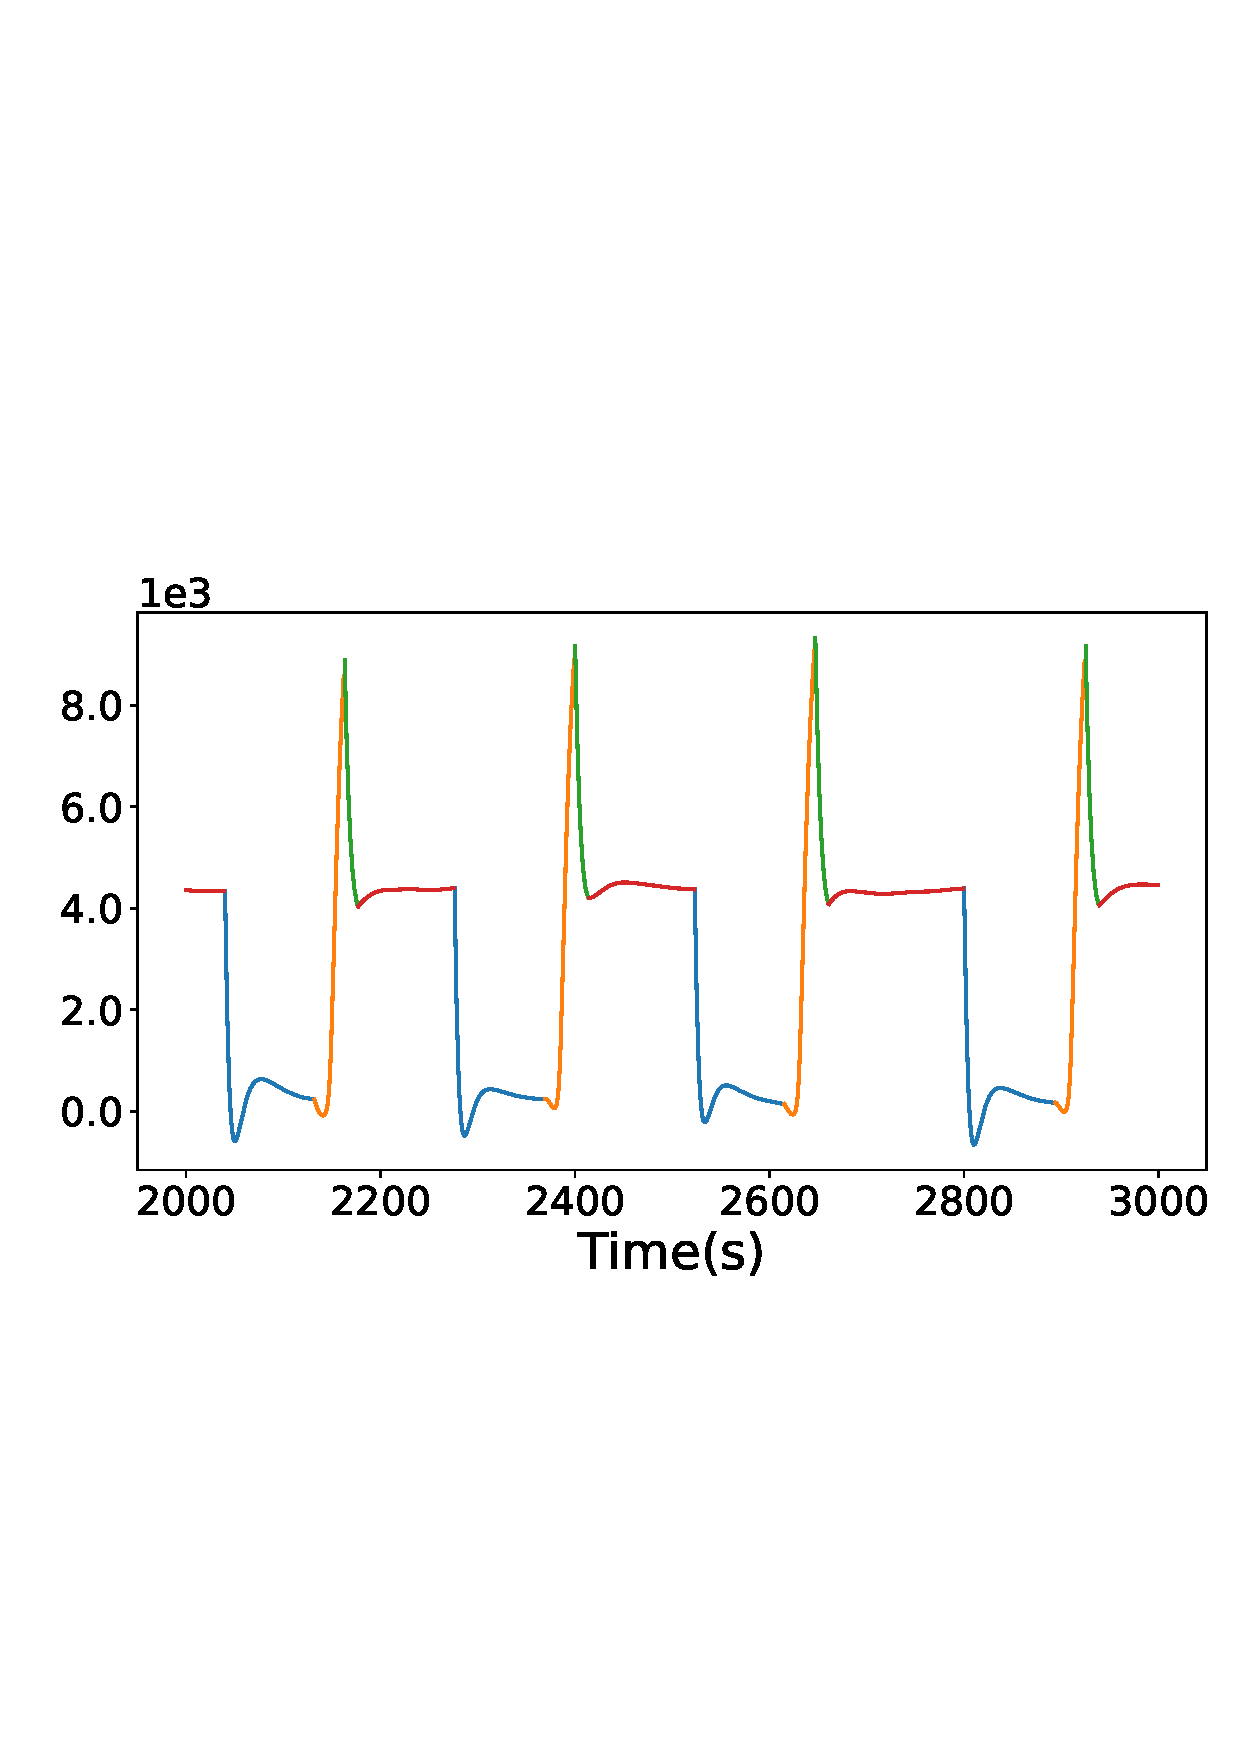
\includegraphics[width=0.45\linewidth]{figures/chapter4/14.pdf}} \hspace{-0.1in}\\
\subfigure[$16^{\circ}C$]{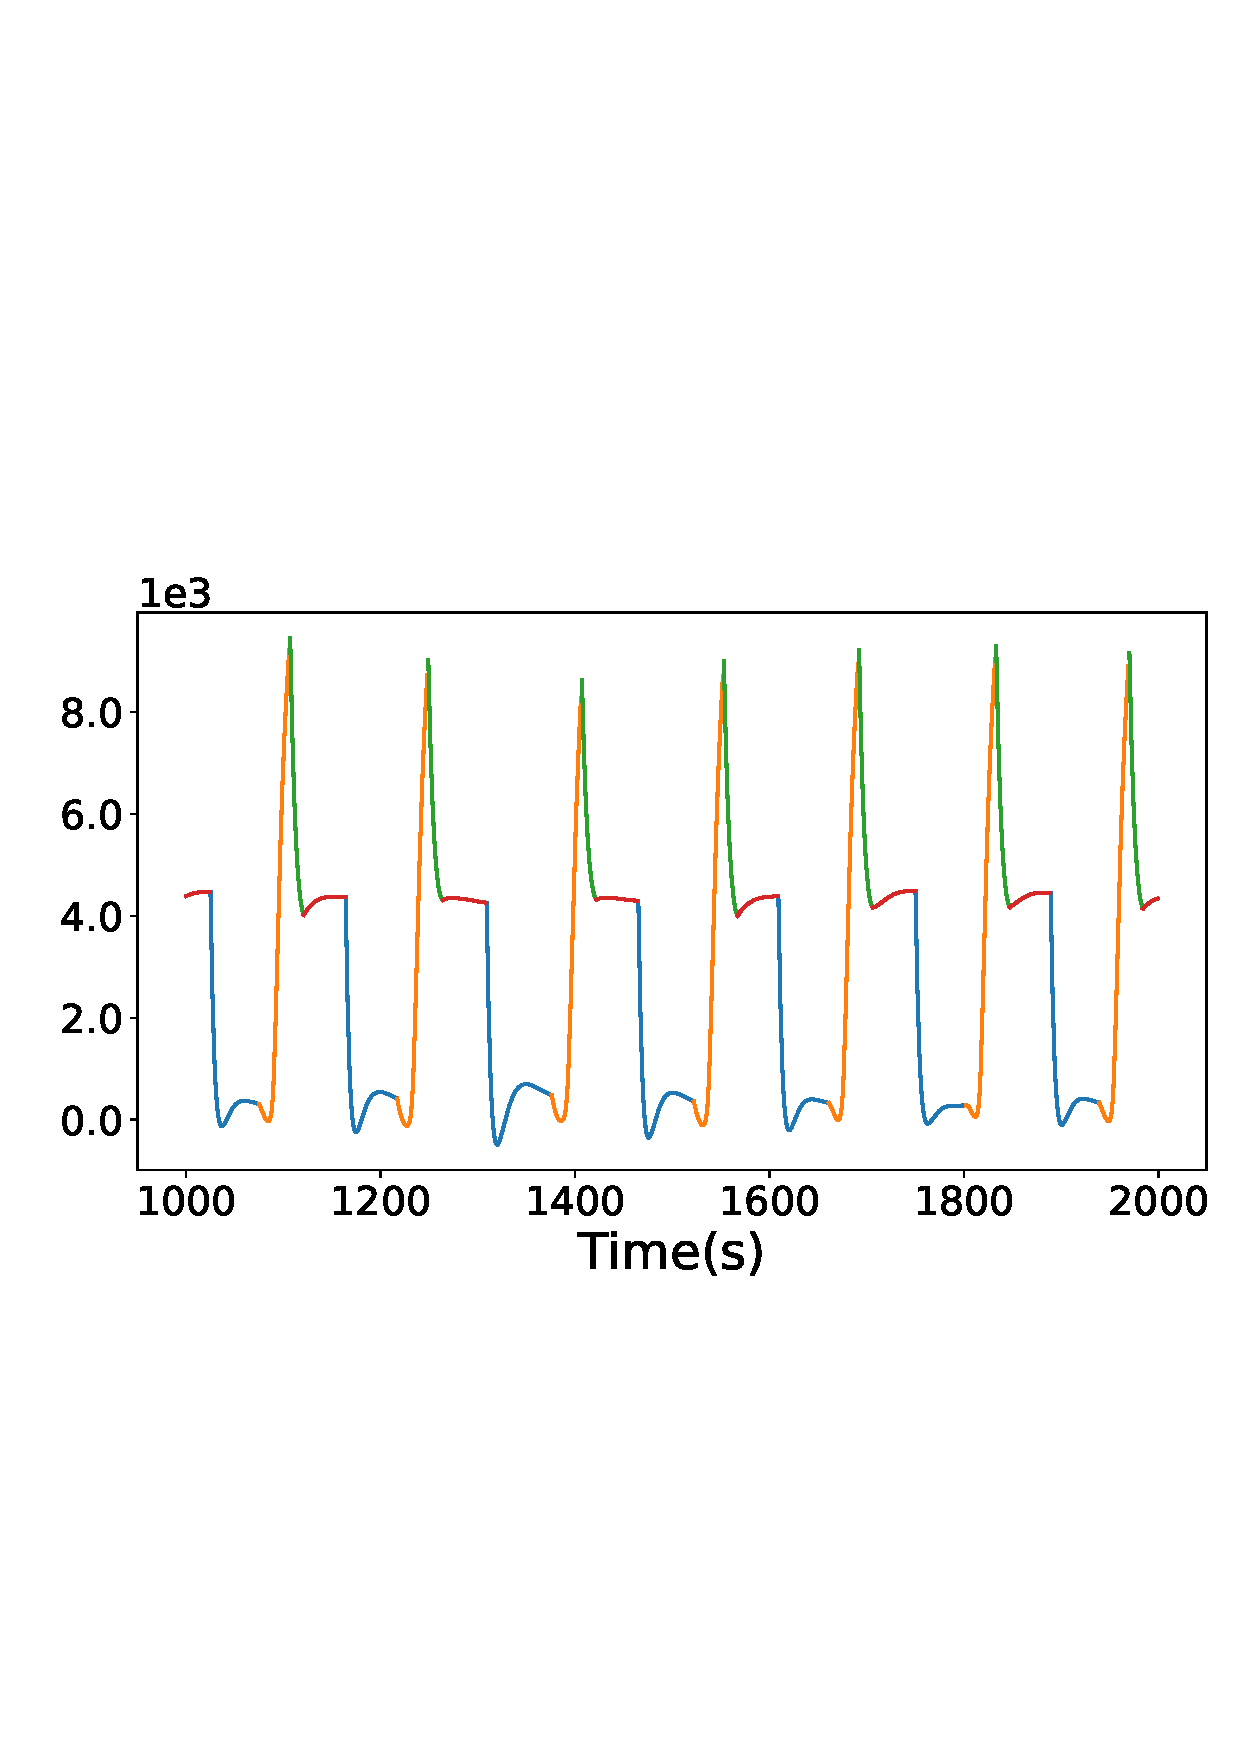
\includegraphics[width=0.45\linewidth]{figures/chapter4/16.pdf}} \hspace{-0.1in}
\subfigure[$18^{\circ}C$]{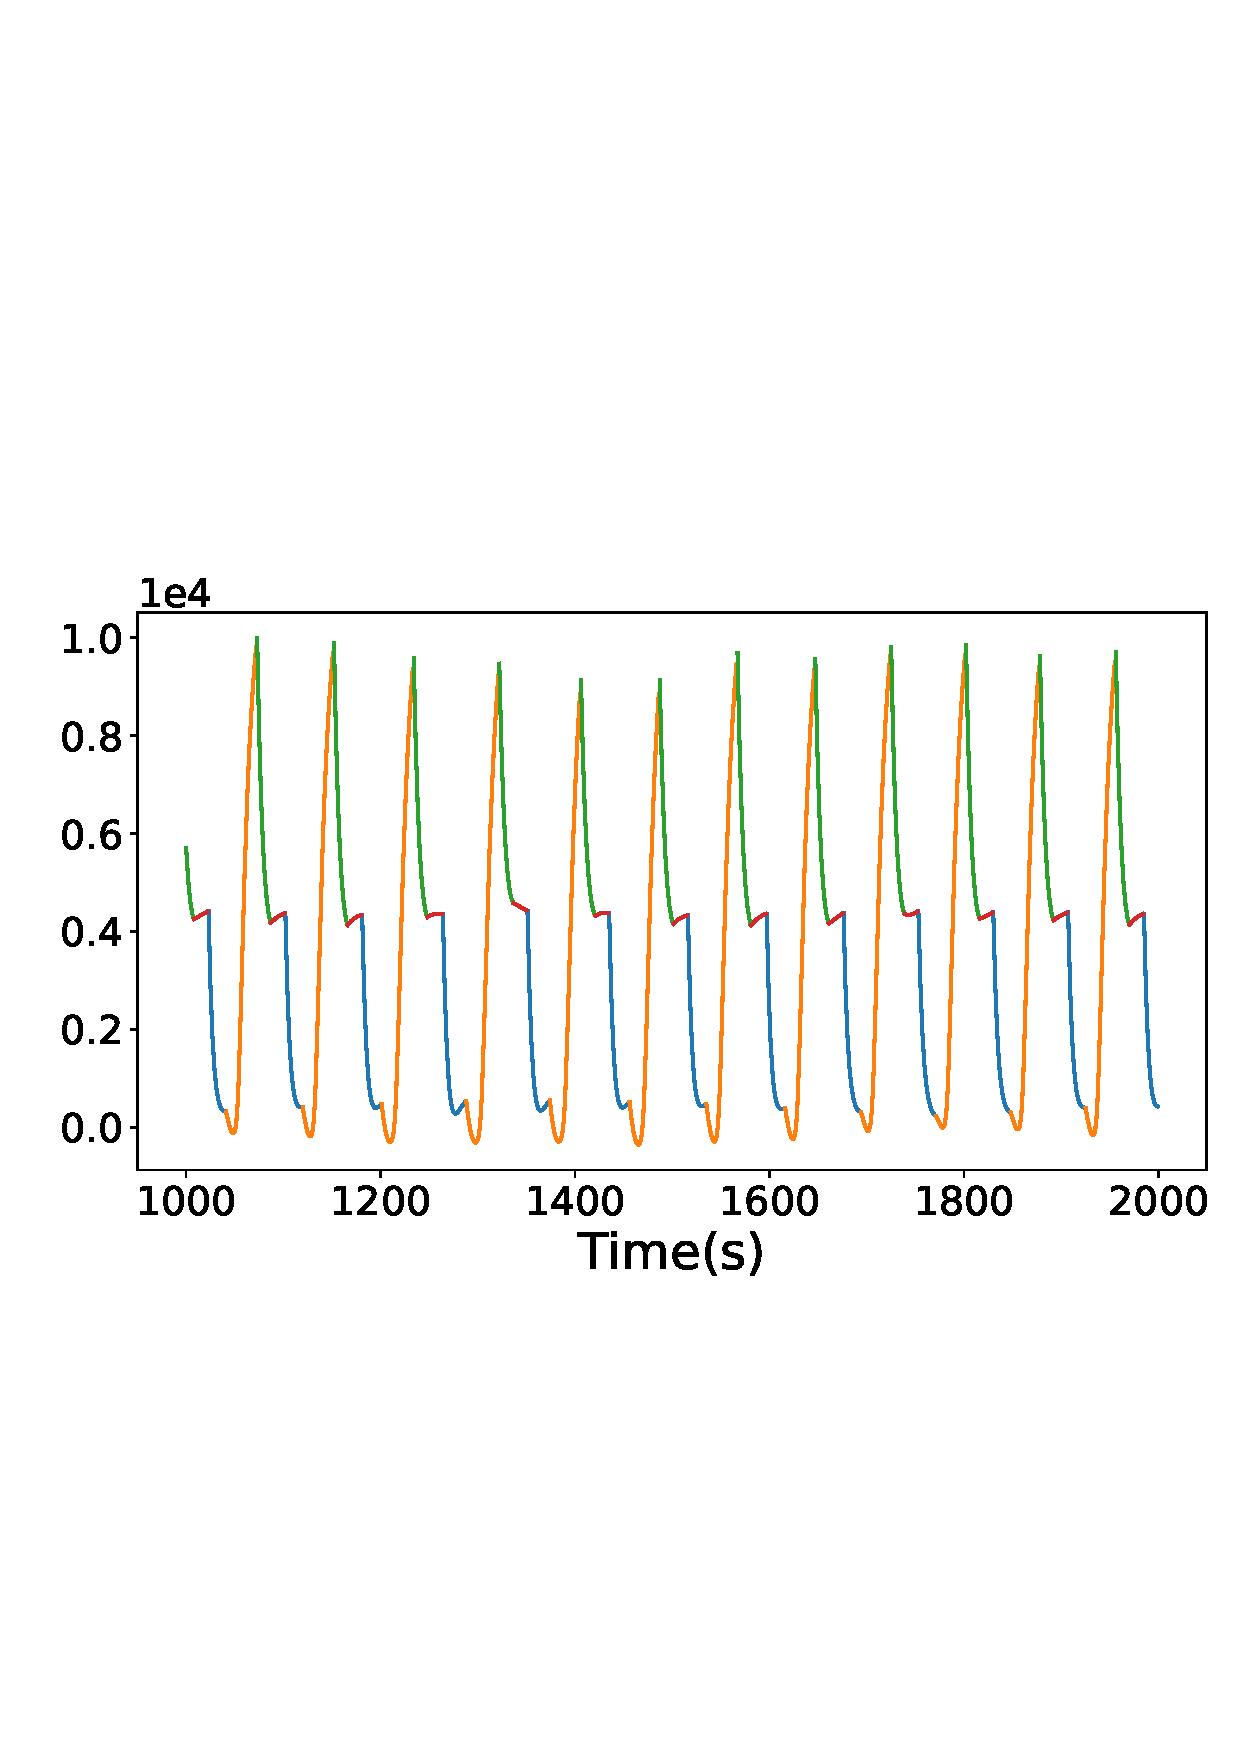
\includegraphics[width=0.45\linewidth]{figures/chapter4/18.pdf}} 
\caption{在不同温度下限设定值下的进气口温度的仿真值}
% \caption{The simulations of instant cooling power under different lower boundary of temperature set points}
%\caption{The simulated instant consumed power with different temperature lower boundaries} %图片标题
\label{fig:lowerbound_simulation}
\end{figure*}

% In Fig.~\ref{fig:temperature}, we evaluate the predicted accumulated power consumption, PUE\footnote{PUE\text{ }=${\text { Total Facility Energy }}/{\text { IT Equipment Energy }}$\cite{song2015data}}, and Coefficient Of Performance (COP)\footnote{COP\text{ }=${\text { Cooling Production }}/{\text { Power consumption }}$\cite{song2015data}} within an hour for different $Ti_{\min}$.
图~\ref{fig:4_temperature}展示了在不同$Ti_{\min}$制冷系统在一小时内的累积能耗预测值,并结合实际热负载绘制了PUE\footnote{PUE\text{ }=${\text {  总能耗 }}/{\text { 设备工作能耗 }}$\cite{song2015data}} 以及性能系数(COP)\footnote{COP\text{ }=${\text {制冷量}}/{\text { 制冷能耗}}$\cite{song2015data}}的变化曲线。
PUE代表整体总能耗(制冷能耗与工作能耗的和)与工作能耗的比。
% PUE is the ratio of the total amount of energy used by a data center facility to the energy delivered to computing equipment.
% The more close PUE is to 1, the more energy-efficient the data center is.
% COP is a ratio of the actual produced cooling to required energy consumption.
PUE越接近1,说明整套制冷系统越节能。
COP是实际产生的制冷量与制冷所需能耗的比值。

% When the lower threshold is increased from ${12}^{\circ} \mathrm{C}$ to ${18}^{\circ} \mathrm{C}$, the total energy consumption declines at first and then gradually goes up after certain points.
当温度下阈值从${12}^{\circ} \mathrm{C}$增加到${18}^{\circ} \mathrm{C}$时,制冷系统总能耗先下降然后逐渐上升。
% Since the higher $Ti_{\min}$ setting narrows the gap between the upper and the lower thresholds, which makes the compressor restart more frequently. Even though the restarting process has short duration, compressor has extremely high power. 
适当增加$Ti_{\min}$时,可以有效地避免过度制冷,从而减少能耗。
但是过度增加$Ti_{\min}$会缩小温度上下限之间的间距,使得压缩机更频繁地重启。虽然重启时间较短,但此时压缩机功耗是极高的。
% As a result, from certain point on, the energy consumption accumulated during compressor restarting process accounts for an important portion, and total energy consumption goes up after that. This certain point is actually the optimal $Ti_{\min}$ that we are searching for.
当达到某一温度后,由于压缩机重新启动所需的能耗占据了制冷系统总能耗的主要部分,此后继续升高$Ti_{\min}$会使总能耗增加,这一拐点就是寻找的最佳$Ti_{\min}$。
当$Ti_{\min}$达到某一温度后,由于压缩机频繁重启增加的能耗与减少过度制冷节省的能耗持平时,此后继续升高$Ti_{\min}$会使总能耗增加。这一拐点就是本项工作希望寻找的最佳$Ti_{\min}$。
% For the three experiments with different heat loads, the optimal $Ti_{\min}$, where the total energy consumption is minimized are marked in Fig.~\ref{fig:energy}. 
对于三个不同热负载的数据集,图~\ref{fig:energy}中标出了使总能耗最小的最佳的$Ti_{\min}$。
% In Fig.~\ref{fig:pue}, the optimal temperature thresholds are consistent with the ones in Fig.~\ref{fig:energy}.
% In Fig.~\ref{fig:cop}, COP decreases with the increase of $Ti_{\min}$. 
% The reason is that frequent on-off operations reduce the time for stable cooling. 
在图~\ref{fig:4_temperature}\subref{fig:pue}中,最佳温度阈值与图~\ref{fig:4_temperature}\subref{fig:energy}中的阈值一致。
在图~\ref{fig:4_temperature}\subref{fig:cop}中,COP随着$Ti_{\min}$的增加不断降低。其原因为频繁的压缩机开闭过程会减少稳定制冷的时间,进而导致单位功耗产生的制冷量下降。
% We take it for granted that the COP is lower when system is unstable.
% When the cooling system runs unstably for a long time, the COP decreases naturally.
% The decline tendency in COP also explains why the required cooling decreases while the energy consumption increases.
COP的下降趋势也解释了为什么提高温度下限值能够使所需的冷气量减少而总制冷能耗却增加。

% 仿真结果如图.~\ref{fig:temperature}所示,曲线中标出了系统达到最小功耗时的温度下限设定值。
与此同时我们发现,最优温度设定点随热负载的增加而增加。因为热负载较高时,制冷系统在\text{On}阶段需要工作更长的时间才能使温度降低到$Ti_{\min}$,变相地增加了制冷阶段在完整工作周期中的占比。
这一发现也在一定程度上表明制冷系统的PUE与制冷、待机两阶段时长的比例具有很强的相关性。

基于仿真实验推导出的最优温度设置点$Ti^*_{\min}$,表~\ref{tab:power_save_percent}展示了优化温度设定点可以节省的功耗百分比。
表~\ref{tab:power_save_percent}展示了基于仿真实验推导出的最优温度设置点$Ti^*_{\min}$以及通过优化温度设定点可以节省的功耗百分比。
根据仿真结果,采用新的温度下限设定值可以节省约6-25\%的能耗,特别对于高热负载情况下的能耗优化是极其显著的。
因为实验\ref{sec:case-study1}中评估了模型预测累积能耗的相对百分比误差小于5\%,可以认为本节对于不同温度下限设定值的仿真结果有足够的可信度。
在未来的工作中,将进一步验证该温度设定策略在实际工业制冷系统中的能耗优化表现。

% The simulations are shown in 图.~\ref{fig:temperature}, and the optimal lower temperature set point, which can achieve the least energy consumption are marked in the curves. 
% It can be found that, optimal temperature set points are varied with the heat load, higher heat load corresponding to higher optimal temperature set points. 
% Based on the inferred optimal set points, the percentage of the saved energy is simulated and shown in \ref{tab:power_save_percent}.
% From results, we find that optimizing the lower boundary set point will produce great energy saving. 
% It is an extremely economical and green improvement of the studied data center, which is supposed to be verified in the future work.

\begin{table}[]
\centering
\caption{能耗优化效果}
\label{tab:power_save_percent}
\begin{tabular}{lcccc}
\hline
\multicolumn{1}{c}{\textbf{不同负载的数据集}} & 1.7k  & 3.8k    & 6.3k  \\ \hline
最优温度设定值(${ }^{\circ} \mathrm{C}$)               & 14   & 15     & 15.5    \\
最大功耗优化比例(\%)              & 6.49 & 10.93  & 25.71\\ \hline
\end{tabular}
\end{table}


% optimized power,best temp set point is the temperature point when the power consumption is the lowest ,max optimized power is compare the lowest power consumption with the truth power consumption



% \begin{table*}[]
% \centering
% \caption{rrse(1.7k)}
% \label{tab:rrse(1.7k)}
% \begin{tabular}{lccc}
% \hline
% \textbf{\%RRSE(1.7k)} & Ti    & PCooling & Power Cooling \\ \hline
% H-ODE                 & 14.32  & 17.34    & 19.37        \\
% ODE-RNN               & 16.33  & 18.86    & 16.79        \\ \hline
% \end{tabular}
% \end{table*}

% \begin{table*}[]
% \centering
% \caption{rrse(3.8k)}
% \label{tab:rrse(3.8k)}
% \begin{tabular}{lccc}
% \hline
% \textbf{RRSE(3.8k)} & Ti    & PCooling & Power Cooling \\ \hline
% H-ODE               & 12.77 & 14.60    & 17.79         \\
% ODE-RNN             & 15.37 & 15.25    & 16.97         \\ \hline
% \end{tabular}
% \end{table*}



% \begin{table*}[]
% \centering
% \caption{rrse(4.2k)}
% \label{tab:rrse(4.2k)}
% \begin{tabular}{lccc}
% \hline
% \textbf{RRSE(4.2k)} & Ti    & PCooling & Power Cooling \\ \hline
% H-ODE               & 13.34 & 15.57    & 18.88         \\
% ODE-RNN             & 17.03 & 18.61    & 17.54         \\ \hline
% \end{tabular}
% \end{table*}

% \begin{table*}[]
% \centering
% \caption{rrse(6.3k)}
% \label{tab:rrse(4.2k)}
% \begin{tabular}{lccc}
% \hline
% \textbf{RRSE(6.3k)} & Ti    & PCooling & Power Cooling \\ \hline
% H-ODE               & 13.07 & 15.65    & 19.29         \\
% ODE-RNN             & 17.75 & 18.61    & 18.23         \\ \hline
% \end{tabular}
% \end{table*}


% \begin{figure}
% \centering
% \subfigure[The time of state-off]{\includegraphics[width=4cm]{figures/chapter4/state1.png}}
% \subfigure[The time of state-on]{\includegraphics[width=4cm]{figures/chapter4/state4.png}}
% \caption{The data of the four data sets are generated at different power of the server, which are 1.7kw, 3.8kw, 4.2kw and 6.3kw respectively. Compare the duration time of system on and off under different power.} %图片标题
% \label{fig:state}  %图片交叉引用时的标签
% \end{figure}

\begin{figure*}[htb]
    \centering
    \subfigure[制冷能耗]{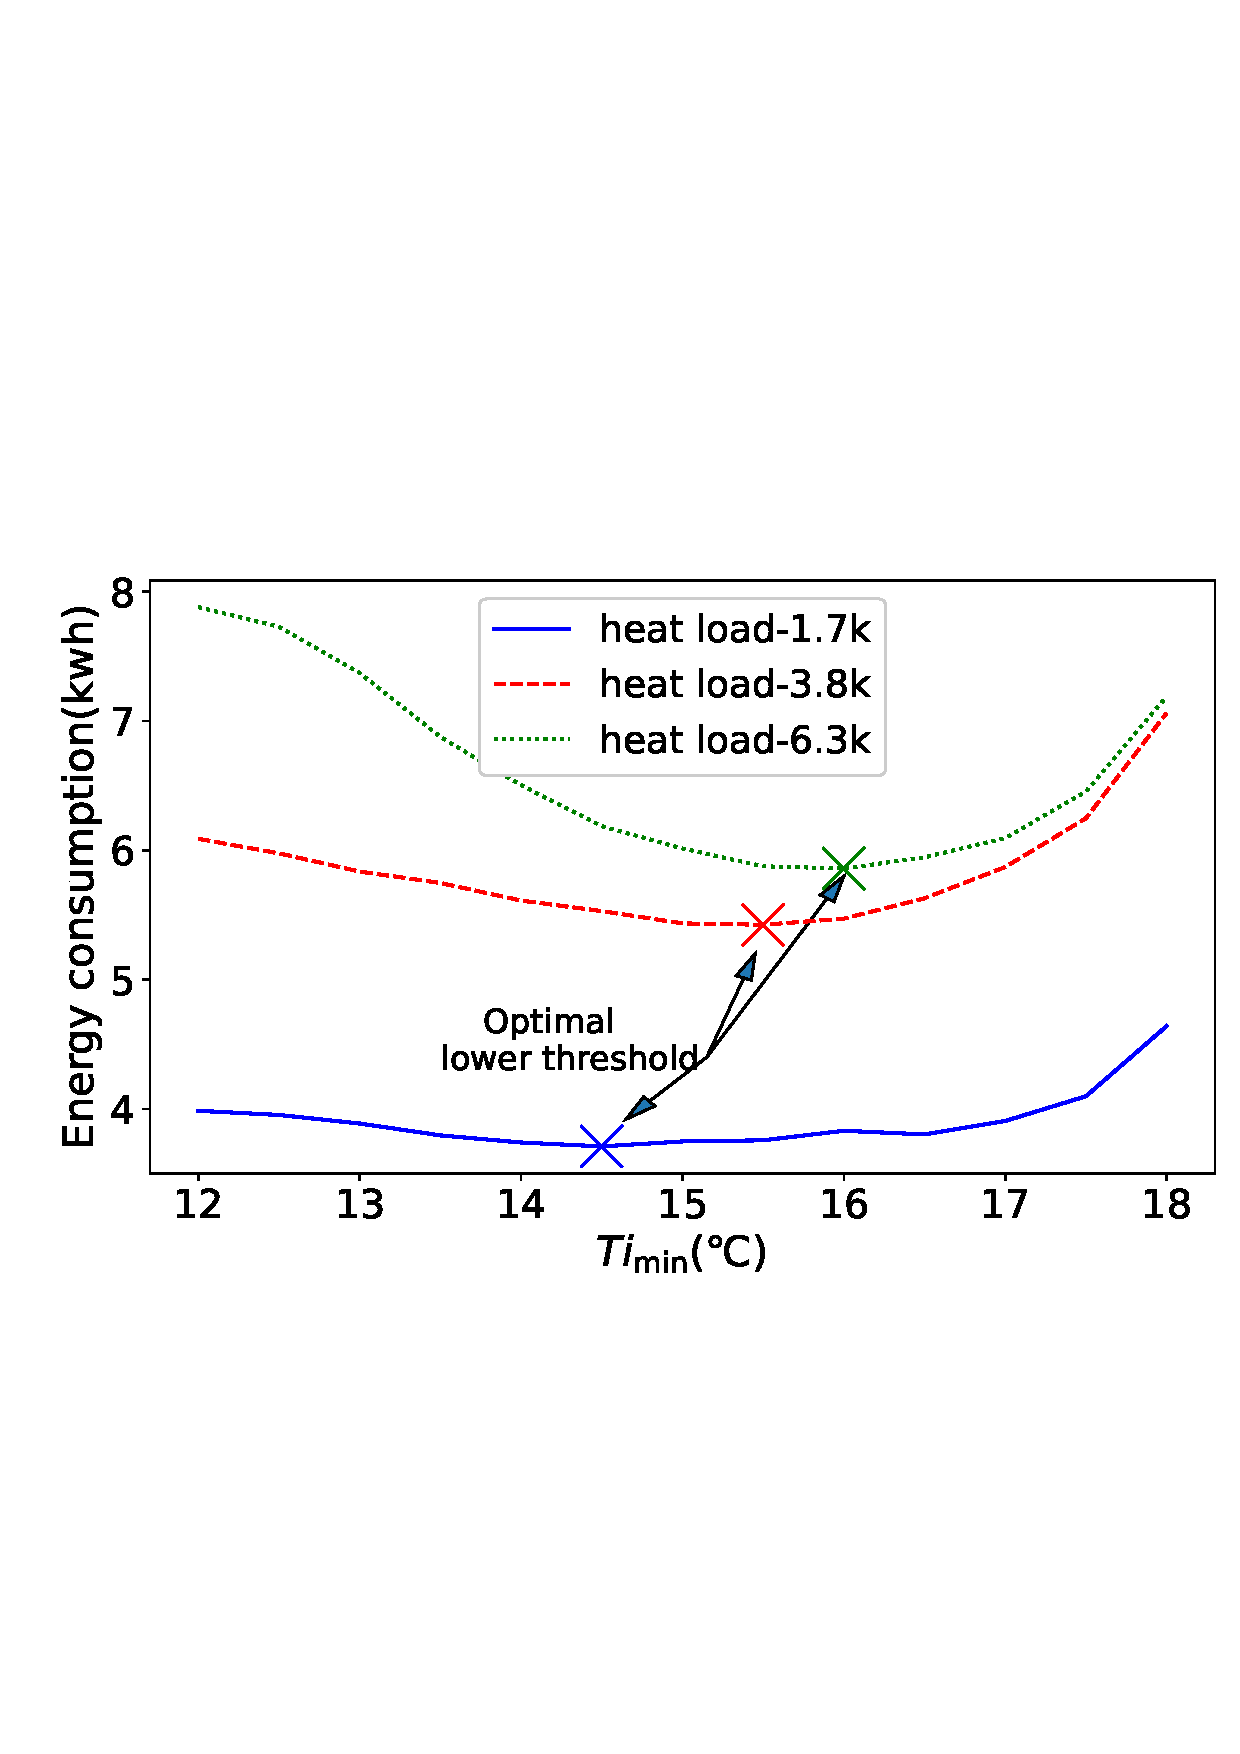
\includegraphics[width=0.7\linewidth]{figures/chapter4/power.pdf}\label{fig:energy}}
    \subfigure[PUE]{\includegraphics[width=0.7\linewidth]{figures/chapter4/pue.pdf}\label{fig:pue}}
    \subfigure[COP]{\includegraphics[width=0.7\linewidth]{figures/chapter4/cop.pdf}\label{fig:cop}}
    % \includegraphics[width=8cm]{figures/temperature.eps}
    \caption{在不同热负载下改变温度设定下限值对功耗、COP、PUE的影响}
    \label{fig:4_temperature}
    % \vspace{-10pt}
\end{figure*}

\section{本章小结}
\label{sec:4_conclusion}
本章针对连续时间周期跳变系统的建模预测问题,提出了一种基于自跳跃常微分方程模型,同时基于该模型构建了用于系统开环预测的编码器-解码器框架。
% 该模型能够对给定历史序列数据中学习系统中不同阶段下的多输入多输出动态特性,通过给定未来的系统输入能够预测系统的未来输出。
该框架能够对给定的历史序列数据进行编码,通过给定系统的未来序列输入,模型能够预测周期跳变系统的未来阶段变化以及系统输出。
% 中学习系统中不同阶段下的多输入多输出动态特性,通过给定未来的系统输入能够预测系统的未来输出。
为了使模型更好地学习跳变系统在不同阶段内的动态特性,AJ-ODE-Net包含了多个层次常微分方程网络, 每个H-ODE-Net能够独立地学习各阶段下的系统动态,并分别建模系统的稳定输出和非稳定输出。同时,AJ-ODE-Net构建阶段转换预测器以指定各个预测时刻所用的H-ODE-Net。
% 作为ODE-Net的扩展,H-ODE-Net中的双层结构分别用于估计隐状态的导数和系统输出的导数,并且对于稳定输出和非稳定输出采用不同的导数模块进行建模。
% 基于AJ设计的阶段转换预测器将系统的先验知识集成为转换规则,以提高模型的预测精度和可解释性。
最后,本章利用所提出的基于AJ-ODE-Net的编码器-解码器框架建模某一工业制冷系统。
与其他方法相比,AJ-ODE-Net能够很好地预测制冷系统温度、功耗变化,并且能够准确地预估阶段转换点。
% Furthermore, we search the optimal lower threshold set points for the inlet temperature for minimizing cooling energy consumption with different heat loads.
此外,
本章依托于训练得到的能耗仿真模型,成功优化了制冷系统的温度下限设定点,有效减少了不同热负荷下的制冷能耗。
% It is shown that up to 25\% energy can be saved by adopting the optimized settings obtained by the simulations.
仿真结果表明,采纳优化后的温度阈值可以节省高达6-25%的制冷能耗。
% The proposed AJ-ODE-Net could be deployed forward to model general continuous-time markov jump systems, future works will be devoted to extend the deterministic stage prediction to markov process.
% 本章所提出的AJ-ODE-Net可以被应用于一般的连续时间马尔科夫跳跃系统的模型中,未来的工作将致力于将确定性的阶段预测扩展到带有随机性的马尔科夫过程。
% Moreover, instead of designing transition rules manually in complex systems, we consider to further develop more intelligent stage labeling solutions based on unsupervised machine learning methods~\cite{10.1145/3097983.3098060}.

在未来的研究工作中,可以尝试将AJ-ODE-Net推广至更通用的马尔科夫连续时间跳变系统,将固定的周期转换过程推广至随机的马尔科夫链。
另外,本文采用自定义状态转移规则的方式对原始系统输出序列进行阶段标注。未来将考虑引入无监督统计学习方法,实现更加智能的自动标注~\cite{10.1145/3097983.3098060}。





% 此外,基于训练得到的仿真模型实现了对于制冷系统的能耗仿真。实验结果表明,当预测时间超过35分钟时,能够基本消除了相位误差的影响,模型能够较为准确地估计预测时间内的系统能耗。另外,该模型能够仿真触发制冷启动的温度设定值对于系统能耗的影响,进而求解使冷却能耗最小的最优温度设定值。通过对不同服务器负载数据进行模拟,给出了不同负载下的最优温度设定,并预估经过优化的设定值能够节省制冷系统能耗约29\%。


% In this paper, a novel deep learning based framework AJ-ODE-Nets is proposed, target at modeling periodic and multi-stage industrial complex systems. It is a MIMO framework, at first place, the framework learns the system behavior and stage transitions during given duration of conditional range, then start to predict required variables with given inputs. AJ-ODE-Net serves as the key module, which takes in inputs, generates hidden states and appoints the system to switch across different ODE-Nets. In order to better characterize different and hybrid physical processes, Hierarchical Neural ODE networks (H-ODE-Net) are adopted to fit different stages of the system, which contains hybrid stationary and non-stationary structure to deal with complex and more general cases. In addition, prior knowledge is integrated and written as transformation rules into the AJ of Stage Transition Predictor. The option allows improving the model interpretability, and exploring system optimization possibilities. With the features mentioned above, AJ-ODE-Net has prominent advantages in simulating multi-stage physical processing. Finally, the proposed AJ-ODE-Net framework is implemented on a cooling system of a running data center. Comparing with other methods, AJ-ODE-Nets achieves better performance in open loop estimation for several operating variables, with accurate results for each stage including the transition point. \\
% Moreover, two applications are realized as use cases. Firstly, the framework is applied to estimate energy consumption for short and long terms cases. Evaluations show that, accurate estimation results can be obtained for prediction duration more than 35 minutes, to get rid of the impact brought by initial points (phrase difference in periodic sequences). Secondly, for the purpose of reducing cooling energy consumption, simulations are conducted by varying lower boundary temperature set points within Stage Transition Predictor to search for the optimal configuration under different heat load
% \chapter{插入参考文献}
% \section{\BibTeX 的使用}
% \BibTeX 是一种格式和一个程序,用于协调LaTeX的参考文献处理。\BibTeX 使用数据库的的方式来管理参考文献. \BibTeX 文件的后缀名为 .bib。 先来看一个例子:
% \begin{quote}
% @article\{name1,\\
% author = \{作者, 多个作者用 and 连接\},\\
% title = \{标题\},\\
% journal = \{期刊名\},\\
% volume = \{卷20\},\\
% number = \{页码\},\\
% year = \{年份\},\\
% abstract = \{摘要, 这个主要是引用的时候自己参考的, 这一行不是必须的\}\\
% \}\\

% @book\{name2,\\
% author ="作者",\\
% year="年份2008",\\
% title="书名",\\
% publisher ="出版社名称"\\
% \}
% \end{quote}
% 说明:第一行@article 告诉 \BibTeX 这是一个文章类型的参考文献,还有其它格式, 例如 article, book, booklet, conference, inbook, incollection, inproceedings,manual, misc, mastersthesis, phdthesis, proceedings, techreport, unpublished 等等。接下来的"name1",就是你在正文中应用这个条目的名称。其它就是参考文献里面的具体内容啦。
% \section{在\LaTeX 中使用\BibTeX }
% 为了在LaTeX中使用BibTeX 数据库, 你必须先做下面三件事情:
% \begin{enumerate}
% \item 设置参考文献的类型 (bibliography style). 标准的为 plain:\\
%   $\backslash$bibliographystyle\{plain\}\\
% 将上面的命令放在 \LaTeX 文档的 $\backslash$begin\{document\}后边. 其它的类型包括:\\
% unsrt – 基本上跟 plain 类型一样,除了参考文献的条目的编号是按照引用的顺序,而不是按照作者的字母顺序。\\
% alpha – 类似于 plain 类型,当参考文献的条目的编号基于作者名字和出版年份的顺序。\\
% abbrv – 缩写格式。
% \item 标记引用 (Make citations). 当你在文档中想使用引用时, 插入\LaTeX 命令$\backslash$cite{引用文章名称}。"引用文章名称" 就是前边定义@article后面的名称.
% \item 告诉LaTeX生成参考文献列表,在 LaTeX 的结束前输入$\backslash$bibliography{bibfile}。这里bibfile 就是你的 BibTeX 数据库文件 bibfile.bib .
% \end{enumerate}

% \section{运行 \BibTeX}
% 分为下面四步:
% \begin{enumerate}
% \item 用LaTeX编译你的 .tex 文件 , 这是生成一个 .aux 的文件, 这告诉 \BibTeX 将使用那些应用;
% \item 用\BibTeX 编译 .bib 文件;
% \item 再次用\LaTeX 编译你的 .tex 文件,这个时候在文档中已经包含了参考文献,但此时引用的编号可能不正确;
% \item 最后用 \LaTeX 编译你的 .tex 文件,如果一切顺利的话, 这是所有东西都已正常了.
% \end{enumerate}

% \section{本论文参考文献格式}
% 北京科技大学博士论文的参考文献要求符合国家标准“GB/T7714-2005文后参考文献著录规则”。本模板中已包含了关于符合此要求的gbt7714-2005.bst文件,只需要将参考文献类型设置为$\backslash$bibliographystyle\{gbt7714-2005\}即可。

